\documentclass{ieeeaccessvi}
%% Bản tiếng Việt của bài 2 (IEEE Access). Chỉ là file khung; nội dung ở các file con:
%%   ieeeaccessvi.cls        bản sao của ieeeaccess.cls với mã chữ T5 (vntex) và nhãn tiếng Việt
%%   t5times.fd, t5formata.fd, t5helvetica.fd, t5giovannistd.fd   ánh xạ font của template sang font T5
%%   preamble.tex            dùng chung với bản tiếng Anh (gói, macro, đường dẫn hình)
%%   frontmatter_vi.tex      tiêu đề, tác giả, tóm tắt, từ khoá
%%   sections_vi/1_introduction.tex, 2_literature_review, 3_theoretical_framework (BQI),
%%   4_methodology, 5_results, 6_discussion (incl. limitations), 7_conclusion, 8_appendices
%%   references.bib          dùng chung với bản tiếng Anh (IEEEtran.bst, thứ tự trích dẫn)
%%   biography_vi.tex        tiểu sử tác giả
%% Không dùng \PARstart (chữ hoa đầu đoạn) vì macro đó cắt rời byte của chữ có dấu.
%% Biên dịch trong thư mục này:
%%   pdflatex access_vi && bibtex access_vi && pdflatex access_vi && pdflatex access_vi
\usepackage[T5]{fontenc}
\usepackage[utf8]{inputenc}
%% Packages, bold-math set-up of the IEEE Access template, graphics path and macros.
%% Input by access.tex before \begin{document}.
\usepackage{cite}
\usepackage{amsmath,amssymb,amsfonts}
\usepackage{graphicx}
\usepackage{textcomp}
\usepackage{booktabs}
\usepackage{url}
\usepackage{bm}
\makeatletter
\AtBeginDocument{\DeclareMathVersion{bold}
\SetSymbolFont{operators}{bold}{T1}{times}{b}{n}
\SetSymbolFont{NewLetters}{bold}{T1}{times}{b}{it}
\SetMathAlphabet{\mathrm}{bold}{T1}{times}{b}{n}
\SetMathAlphabet{\mathit}{bold}{T1}{times}{b}{it}
\SetMathAlphabet{\mathbf}{bold}{T1}{times}{b}{n}
\SetMathAlphabet{\mathtt}{bold}{OT1}{pcr}{b}{n}
\SetSymbolFont{symbols}{bold}{OMS}{cmsy}{b}{n}
\renewcommand\boldmath{\@nomath\boldmath\mathversion{bold}}}
\makeatother

\graphicspath{{../outputs/paper/eeg/}{../outputs/paper/realdata/}{../outputs/paper/osf3uszv/}}

\newcommand{\kinh}{k_{\mathrm{inh}}}
\newcommand{\kd}{k_{d}}
\newcommand{\sA}{\sigma_{A}}
\newcommand{\sPhi}{\sigma_{\Phi}}
\newcommand{\rA}{r_{A}}
\newcommand{\rPhi}{r_{\Phi}}
\newcommand{\rQ}{r_{Q}}
\newcommand{\CRB}{\mathrm{CRB}}
\newcommand{\RMSE}{\mathrm{RMSE}}
\newcommand{\QoC}{\mathrm{QoC}}
\newcommand{\dd}{\,\mathrm{d}}
\newcommand{\thetav}{\boldsymbol{\theta}}
\newcommand{\xv}{\mathbf{x}}
\newcommand{\yv}{\mathbf{y}}
\newcommand{\Cov}{\operatorname{Cov}}
\newcommand{\diag}{\operatorname{diag}}
% notation of the BQI paper (D. Q. Vu, paper/bqi_paper.pdf)
\newcommand{\ADMN}{A_{\mathrm{DMN}}}
\newcommand{\kint}{k_{\mathrm{int}}}
\newcommand{\kspont}{k_{\mathrm{spont}}}
\newcommand{\Amax}{A_{\max}}
\newcommand{\PCI}{\mathrm{PCI}}
\newcommand{\LZC}{\mathrm{LZC}}
\newcommand{\KL}{\mathrm{KL}}

% Reference [BQI] (D. Q. Vu, paper/bqi_paper.pdf) has no DOI or preprint yet: its entry in the
% reference list is printed in red until it does. Delete this block once the DOI is in references.bib.
\makeatletter
\def\BQI@key{BQI}
\newcommand{\BQI@wrapbibitem}[1]{\normalcolor\BQI@origbibitem{#1}\def\BQI@this{#1}%
  \ifx\BQI@this\BQI@key\color{red}\fi}
\AtBeginDocument{\let\BQI@origbibitem\bibitem\let\bibitem\BQI@wrapbibitem}
\makeatother


\begin{document}
%% Khối tiêu đề, tóm tắt và từ khoá (bản tiếng Việt). Được access_vi.tex \input ngay sau \begin{document}.
%% TODO: danh sách tác giả, e-mail và DOI trước khi nộp.
\history{Ngày công bố xxxx 00, 0000, ngày của phiên bản hiện tại xxxx 00, 0000.}
\doi{10.1109/ACCESS.2026.0000000}

\title{Từ phương trình đến điện cực: kiểm định có đăng ký trước mô hình Bộ não như một giao diện truy vấn của thiền trên hai bộ dữ liệu EEG mở}
% TODO: xác nhận danh sách tác giả và đơn vị trước khi nộp (cùng khối như bài đồng hành).
\author{\uppercase{Dung Vu}\authorrefmark{1}}
\address[1]{Trường Đại học Phenikaa, Hà Nội 12116, Việt Nam (e-mail: [e-mail cơ quan])}
\tfootnote{Nghiên cứu được thực hiện tại Trường Đại học Phenikaa, Hà Nội. Mọi tính toán chạy trên máy tính cá nhân; không nhận tài trợ bên ngoài.}

\markboth
{Vu: Từ phương trình đến điện cực: kiểm định mô hình BQI của thiền trên EEG}
{Vu: Từ phương trình đến điện cực: kiểm định mô hình BQI của thiền trên EEG}

\corresp{Tác giả liên hệ: Dung Vu (e-mail: [e-mail cơ quan]).}

\begin{abstract}
Các mô hình động lực nối hoạt động của mạng chế độ mặc định, mức tích hợp thông tin và chất lượng thiền do người tập tự báo cáo ngày càng được đề xuất nhiều, và một phân tích thiết kế dựa trên thông tin Fisher chính xác của một mô hình không gian trạng thái tuyến tính--Gauss gần đây đã dự đoán mô hình như vậy có thể được ước lượng chính xác đến đâu từ điện não đồ (EEG) lấy mẫu trải nghiệm. Các dự đoán đó có đúng trên bản ghi thật hay không thì chưa được kiểm tra. Chúng tôi fit mô hình lên hai bộ dữ liệu EEG lấy mẫu trải nghiệm mở của hai phòng thí nghiệm khác nhau, ds001787 (24 người tập, 40 phiên, 983 lần hỏi tự chấm) và OSF 3uszv (58 người, 58 phiên, 2\,258 lần hỏi), theo hai bản đăng ký trước được khoá bằng mã băm và bốn cổng kiểm tra tự động cho mỗi bộ. Trên cả hai bộ, sai số tương đối của hằng số tốc độ của mạng chế độ mặc định được dự đoán trước khi khoá gần với sai số chuẩn Fisher tại ước lượng và với sai số bootstrap tham số (9,1; 9,9 và 9,7 phần trăm trên ds001787; 6,7; 8,5 và 8,8 phần trăm trên OSF 3uszv), trong khi sai số theo thông tin quan sát của kênh công suất alpha vượt giá trị Fisher, một dấu hiệu sai đặc tả không xuất hiện trên dữ liệu mô phỏng từ fit. Không đại diện EEG nào cải thiện dự đoán ngoài mẫu của điểm tự chấm so với các mô hình rỗng trên bộ nào. Bản thân các hằng số tốc độ không lặp lại: hằng số thời gian của mạng chế độ mặc định là 0,76 phút trên ds001787 và 7,1 phút trên OSF 3uszv, và một mô phỏng cho thấy fit Ornstein--Uhlenbeck trả về thang thời gian trội của bất kỳ đặc trưng nào được đưa vào. Các phân tích thiết kế kiểu này đáng tin về độ chính xác mà chúng hứa hẹn, nhưng không đáng tin về ý nghĩa của các tham số ước lượng từ đại diện chưa hiệu chuẩn.
\end{abstract}

\begin{keywords}
Bộ lọc Kalman, cận Cramér--Rao, đăng ký trước, điện não đồ, lấy mẫu trải nghiệm, mạng chế độ mặc định, mô hình không gian trạng thái, sai đặc tả mô hình, thiền, thông tin Fisher.
\end{keywords}

\titlepgskip=-21pt

\maketitle


%% I. Giới thiệu: bối cảnh, vấn đề, khoảng trống, câu hỏi nghiên cứu, đóng góp, bố cục. Được access_vi.tex \input.
\section{Giới thiệu}
\label{sec:intro}
Nghiên cứu về thiền đã chuyển từ khác biệt trung bình giữa người thiền và nhóm đối chứng sang mô hình hoá \emph{động lực} của một phiên: sự luân phiên giữa chú ý tập trung, lang thang tâm trí và siêu nhận thức \cite{Hasenkamp2012,Lutz2008,Christoff2016}, sự điều tiết mạng chế độ mặc định (DMN) \cite{Raichle2001,Brewer2011,Garrison2015}, và các cách giải thích tính toán theo xử lý dự đoán \cite{Laukkonen2021,SandvedSmith2021}. Khung lý thuyết Bộ não như một giao diện truy vấn (Brain as a Query Interface, BQI) của Vũ \cite{BQI} viết động lực đó thành phương trình vi phân nối hoạt động DMN, thông tin tích hợp $\Phi$ và chất lượng ý thức (QoC) do người tập báo cáo, fit các tốc độ và hệ số khuếch đại từ dữ liệu phân tích gộp, và đề xuất điều khiển chúng bằng một giao diện não--máy vòng kín \cite[Mục~7.2, 9.3 và 10.1]{BQI}; đây là nền tảng lý thuyết của nghiên cứu này (Mục~\ref{sec:theory}). Các mô hình kiểu này hứa hẹn những đại lượng ước lượng được từ dữ liệu, như tốc độ DMN bị ức chế và trọng số của mỗi trạng thái ẩn trong báo cáo, và được đưa ra làm nền cho neurofeedback dựa trên mô hình \cite{Sitaram2017}.

Liệu các đại lượng đó có ước lượng được từ loại dữ liệu mà nghiên cứu thiền thực sự thu, EEG liên tục và vài lần hỏi tự chấm mỗi phiên, là một câu hỏi riêng. Trong bài đồng hành \cite{companion}, chúng tôi thay hệ phương trình của BQI bằng một mô hình không gian trạng thái tuyến tính--Gauss (M1) và dùng thông tin Fisher kỳ vọng chính xác của nó để tính cần bao nhiêu người, phiên dài bao nhiêu, hỏi dày bao nhiêu và đặc trưng EEG sạch đến đâu để ước lượng mỗi tham số đến một độ chính xác cho trước. Phân tích thiết kế đó mới chỉ được kiểm chứng trên dữ liệu mô phỏng. Chưa nghiên cứu nào kiểm phân tích thiết kế như vậy trên bản ghi thật, so các ước lượng với giá trị mà BQI rút ra từ tài liệu, hay hỏi các tham số ước lượng được có chuyển được từ phòng thí nghiệm này sang phòng thí nghiệm khác không (Mục~\ref{sec:gap}).

Trả lời sạch các câu hỏi này không dễ. Các đặc trưng EEG đứng thay cho DMN và cho $\Phi$ là đại diện chưa có ánh xạ hiệu chuẩn sang biến trạng thái; một phần ba bản ghi có thể bị thiếu; mô hình có thể sai đặc tả theo cách mà một cận không lường trước được; và một phân tích có nhiều lựa chọn tự do (đặc trưng, quy tắc nhiễu giả, mô hình rỗng, tiêu chí loại) có thể hậu thuẫn gần như mọi kết luận sau khi đã xem dữ liệu. Vì vậy chúng tôi đăng ký trước toàn bộ kế hoạch phân tích cho mỗi bộ trong hai bộ dữ liệu mở, khoá bằng mã băm SHA-256 trước khi xem EEG \cite{Nosek2018}, tổ chức pipeline thành một chuỗi cổng kiểm tra tự động từ chối chạy tiếp khi điều kiện tiên quyết không đạt, và báo cáo mọi phân tích đã khoá dù có ủng hộ dự đoán hay không.

\subsection{Câu hỏi nghiên cứu}
\begin{enumerate}
  \item[RQ1] \emph{Độ chính xác.} Trên một thiết kế lấy mẫu trải nghiệm thật, với lịch hỏi không đều, epoch thiếu và loại nhiễu giả, sai số tương đối của tham số khó nhất, hằng số tốc độ DMN $\kinh$, có gần cận Cramér--Rao (CRB) tính từ lịch hỏi thật trước khi xem EEG không?
  \item[RQ2] \emph{Dự đoán.} Một mô hình xác định được về nguyên tắc, fit lên EEG liên tục và các báo cáo thưa, có dự đoán báo cáo ngoài mẫu tốt hơn các mô hình bỏ qua động lực không?
  \item[RQ3] \emph{Khớp với BQI.} Các hằng số tốc độ, hệ số ghép và hệ số khuếch đại ước lượng được có khớp với các giá trị mà BQI fit từ dữ liệu phân tích gộp không?
  \item[RQ4] \emph{Lặp lại.} Các tham số ước lượng được có cùng nghĩa giữa các bản ghi của các phòng thí nghiệm khác nhau, với bộ khuếch đại, montage, lịch hỏi và thang điểm khác nhau không?
\end{enumerate}

\subsection{Đóng góp}
\begin{enumerate}
  \item Phép thử đầu tiên, theo hiểu biết của chúng tôi, của một phân tích thiết kế bằng thông tin Fisher cho mô hình động lực của thiền trên EEG lấy mẫu trải nghiệm thật, trên hai bộ dữ liệu mở độc lập, ds001787 \cite{Brandmeyer2018,Delorme2024ds} và OSF 3uszv \cite{RodriguezLarios2021}, theo hai bản đăng ký trước đã khoá và tám cổng kiểm tra.
  \item Một cách báo cáo ba con số sai số, CRB tính trước khi khoá, sai số chuẩn Fisher tại ước lượng và sai số bootstrap tham số, cùng với sai số theo thông tin quan sát và so sánh với dữ liệu mô phỏng từ fit. Trên cả hai bộ, ba con số đầu khớp nhau với hằng số tốc độ DMN, và con số thứ tư để lộ sai đặc tả của kênh công suất alpha \cite{White1982}.
  \item Một kiểm định ngoài mẫu đã đăng ký trước của mô hình so với ba mô hình rỗng, cho thấy không đại diện EEG nào mang thông tin về báo cáo ngoài phụ thuộc chuỗi của chính báo cáo, trên cả hai bộ.
  \item Một phép so sánh các ước lượng với giá trị tham số của BQI, cùng các kiểm tra lặp lại đã đăng ký trước giữa hai bộ, cho thấy các hằng số tốc độ và khác biệt nhóm giữa người thiền lâu năm và người mới không chuyển được từ bộ này sang bộ kia, kèm một mô phỏng giải thích vì sao: fit Ornstein--Uhlenbeck trả về thang thời gian trội của đặc trưng được đưa vào.
  \item Một pipeline tái tạo được hoàn toàn (mỗi bước một lệnh, có checkpoint, 114 unit test) cùng cả hai bản đăng ký trước, khoá và hồ sơ các cổng.
\end{enumerate}

Phần còn lại của bài theo bố cục thông thường của một bài nghiên cứu. Mục~\ref{sec:litreview} tổng quan tài liệu về mô hình động lực của thiền, khung BQI, các chỉ dấu EEG của hoạt động DMN và của tích hợp, khả năng xác định và thiết kế thí nghiệm cho mô hình động lực, và đăng ký trước, rồi nêu khoảng trống nghiên cứu. Mục~\ref{sec:theory} trình bày khung lý thuyết: mô hình BQI với các phương trình của nó, dẫn xuất mô hình ước lượng được M1 và các dự đoán của BQI cho các đại lượng được ước lượng. Mục~\ref{sec:methods} trình bày phương pháp: thiết kế nghiên cứu, mô hình, giả thuyết, dữ liệu, đăng ký trước, tiền xử lý và phân tích thống kê. Mục~\ref{sec:results} báo cáo kết quả, Mục~\ref{sec:discussion} thảo luận chúng cùng các hạn chế của nghiên cứu, và Mục~\ref{sec:conclusion} kết luận và nêu hướng tiếp theo.

%% II. Tổng quan tài liệu và khoảng trống nghiên cứu. Được access_vi.tex \input.
\section{Tổng quan tài liệu}
\label{sec:litreview}

\subsection{Từ khác biệt nhóm đến động lực của một phiên}
Các nghiên cứu hình ảnh thần kinh đầu tiên về thiền so sánh giữa các nhóm: người thiền lâu năm có hoạt động DMN giảm khi thực hành và kết nối DMN thay đổi \cite{Brewer2011,Garrison2015}, và một phân tích gộp 78 nghiên cứu hình ảnh chức năng vẽ bản đồ các vùng được huy động bởi các kiểu thiền khác nhau \cite{Fox2016}. Các công trình sau chuyển sang động lực bên trong một phiên. Hasenkamp và cộng sự \cite{Hasenkamp2012} chia thực hành chú ý tập trung thành một chu kỳ gồm lang thang tâm trí, nhận ra lang thang, chuyển chú ý và duy trì tập trung; Lutz và cộng sự \cite{Lutz2008} mô tả chú ý tập trung và quan sát mở như hai chiến lược điều tiết chú ý; và Christoff và cộng sự \cite{Christoff2016} coi lang thang tâm trí là suy nghĩ tự phát được định hình bởi các ràng buộc có chủ đích và tự động. Các cách giải thích theo xử lý dự đoán mô tả thiền như một sự làm phẳng dần hệ thứ bậc dự đoán \cite{Laukkonen2021}, và một mô hình suy luận chủ động mô phỏng siêu nhận thức và kiểm soát chú ý trong chú ý tập trung \cite{SandvedSmith2021}. Các cách giải thích này mang tính định tính hoặc là mô hình sinh, và không cách nào nêu các tham số của nó ước lượng được chính xác đến đâu từ dữ liệu mà nghiên cứu thiền thu thập.

\subsection{Khung lý thuyết Bộ não như một giao diện truy vấn}
Trong các cách giải thích động lực, khung BQI của Vũ \cite{BQI} là khung viết động lực của một phiên thành một mô hình tường minh có tham số: nó nối hoạt động DMN, thông tin tích hợp và QoC do người tập báo cáo qua một hệ ODE có tốc độ và hệ số khuếch đại fit từ dữ liệu phân tích gộp, và đề xuất điều khiển chúng bằng một giao diện não--máy vòng kín \cite[Mục~7, 9 và 10]{BQI}. Phần tổng hợp tài liệu của BQI cho biết tín hiệu BOLD của DMN giảm gộp 39,4\,\% qua 16 nghiên cứu ($d=1{,}70$) và hoạt động DMN tương quan nghịch mạnh với QoC ($r=-0{,}89$) \cite[Mục~7.3--7.4]{BQI}. Trong bài đồng hành \cite{companion}, chúng tôi đã chỉ ra rằng phương trình QoC của BQI không có mức dừng và thay hệ bằng mô hình không gian trạng thái M1. BQI là nền tảng lý thuyết của nghiên cứu này; Mục~\ref{sec:theory} trình bày các phương trình của nó và dẫn ra M1 từ đó.

\subsection{Chỉ dấu EEG của hoạt động DMN và của tích hợp}
DMN được xác định từ chụp cắt lớp phát xạ positron và fMRI \cite{Raichle2001}, và các tương ứng EEG của nó là gián tiếp. Các nghiên cứu ghi đồng thời EEG--fMRI liên hệ dao động tự phát của công suất các dải tần với các mạng trạng thái nghỉ: công suất alpha đồng biến âm với một mạng chú ý trán--đỉnh và công suất beta 17--23~Hz đồng biến dương với các vùng của mạng mặc định \cite{Laufs2003}, và mỗi mạng trạng thái nghỉ có một tổ hợp nhịp EEG riêng, trong đó DMN gắn với công suất alpha và beta \cite{Mantini2007}. Vì vậy công suất alpha vùng sau cùng lắm là một đại diện gián tiếp của hoạt động DMN, và được dùng đúng như thế ở đây. Trong nghiên cứu thiền, một tổng quan hệ thống gắn chánh niệm với công suất alpha và theta tăng \cite{Lomas2015}; lang thang tâm trí khi tập trung vào hơi thở đi kèm công suất delta và theta nhiều hơn, alpha và beta ít hơn \cite{Braboszcz2011}; người tập lâu năm báo cáo ít lang thang tâm trí hơn, với các tương quan EEG của trạng thái được báo cáo \cite{Brandmeyer2018}; và khác biệt phổ giữa thiền và lang thang tâm trí không giống nhau ở người thiền lâu năm và người mới \cite{RodriguezLarios2021}. BQI coi công suất theta tăng là dấu hiệu phổ đặc trưng của thiền lâu năm \cite[Phụ lục~B.2]{BQI}. Về tích hợp, bản thân $\Phi$ không tính được cho hệ cỡ bộ não; chỉ số độ phức tạp nhiễu loạn nén đáp ứng của vỏ não với kích thích từ xuyên sọ bằng thuật toán Lempel--Ziv \cite{Casali2013}, độ phức tạp Lempel--Ziv của EEG tự phát giảm khi gây mê bằng propofol \cite{Schartner2015}, và số mũ aperiodic của phổ công suất là một phương án dựa trên phổ \cite{Donoghue2020}. BQI dùng chỉ số độ phức tạp làm đại diện cho $\Phi$ và báo cáo giá trị cao hơn ở người thiền lâu năm \cite[Mục~6.3]{BQI}.

\subsection{Khả năng xác định và thiết kế thí nghiệm cho mô hình động lực}
Liệu các tham số của một mô hình động lực có xác định được từ dữ liệu không nhiễu hay không là câu hỏi về khả năng xác định cấu trúc \cite{Bellman1970}; trong một mô hình tham số chính quy, một điểm xác định được cục bộ khi và chỉ khi ma trận thông tin không suy biến tại đó \cite{Rothenberg1971}. Khả năng xác định thực hành hỏi liệu dữ liệu hữu hạn, có nhiễu có xác định được tham số không, và hợp lý profile là công cụ chuẩn cho câu hỏi này \cite{Raue2009,Wieland2021}. Cận Cramér--Rao \cite{Rao1945,Cramer1946} biến thông tin Fisher thành cận dưới của phương sai của mọi ước lượng không chệch và là nền của thiết kế thí nghiệm tối ưu trong sinh học hệ thống \cite{Kreutz2009}. Với một quá trình ẩn tuyến tính--Gauss được lấy mẫu không đều, bộ lọc Kalman cho hàm hợp lý chính xác \cite{Kalman1960,Harvey1989,Durbin2012}. Khi mô hình sai, thông tin quan sát và thông tin kỳ vọng tách nhau, đó là cơ sở của phép chẩn đoán sai đặc tả dùng ở đây \cite{White1982}. Các công cụ này chưa được áp dụng cho thiết kế lấy mẫu trải nghiệm trong nghiên cứu thiền trước bài đồng hành \cite{companion}, vốn làm điều đó trên mô phỏng.

\subsection{Lấy mẫu trải nghiệm, đăng ký trước và lặp lại}
Lấy mẫu trải nghiệm bằng lần hỏi là cách chuẩn để đo lang thang tâm trí, và cách đặt câu hỏi và chọn thời điểm hỏi làm thay đổi tỉ lệ được báo cáo \cite{Weinstein2018}. Một dự án lặp lại quy mô lớn cho thấy chỉ khoảng một phần ba hiệu ứng tâm lý học đã công bố lặp lại được với kết quả có ý nghĩa \cite{OSC2015}, và đăng ký trước tách phân tích khẳng định khỏi phân tích khám phá bằng cách cố định kế hoạch trước khi xem dữ liệu \cite{Nosek2018}. Các bộ dữ liệu EEG lấy mẫu trải nghiệm mở \cite{Delorme2024ds,RodriguezLarios2021} nay cho phép kiểm định độc lập, có đăng ký trước, một mô hình mà không cần thu dữ liệu mới.

\subsection{Khoảng trống nghiên cứu}
\label{sec:gap}
Từ tổng quan trên có ba khoảng trống. Thứ nhất, chưa phân tích thiết kế nào cho một mô hình động lực của thiền được kiểm trên EEG lấy mẫu trải nghiệm thật; phân tích của bài đồng hành là \emph{in silico}. Thứ hai, các giá trị tham số của BQI được fit từ các tóm tắt phân tích gộp của tương phản fMRI và tương quan cắt ngang \cite[Mục~7.2--7.5]{BQI} và chưa bao giờ được ước lượng từ chuỗi thời gian EEG của từng phiên, trong khi chính các đại diện EEG của DMN và của $\Phi$ còn chưa được hiệu chuẩn. Thứ ba, chưa hằng số tốc độ nào của một mô hình thiền được lặp lại giữa các phòng thí nghiệm theo một kế hoạch đã đăng ký trước. Nghiên cứu này giải quyết ba khoảng trống đó bằng các câu hỏi nghiên cứu RQ1--RQ4.

%% III. Khung lý thuyết: mô hình BQI của Vũ Quang Dũng (paper/bqi_paper.pdf), các phương trình,
%% dẫn xuất mô hình ước lượng được M1 và các dự đoán lý thuyết. Được access_vi.tex \input.
%% Số phương trình, mục, bảng và thuật toán trong \cite[...]{BQI} là số của bài đó.
\section{Khung lý thuyết}
\label{sec:theory}
Nền tảng lý thuyết của nghiên cứu này là mô hình Bộ não như một giao diện truy vấn (BQI) của Vũ \cite{BQI}. Mục này trình bày các phần của BQI mà phân tích dựa vào, kèm số phương trình, mục, bảng và thuật toán của \cite{BQI}, dẫn ra từ đó mô hình không gian trạng thái ước lượng được M1, và liệt kê các dự đoán mà BQI đưa ra cho các đại lượng được ước lượng ở đây.

\subsection{Luận đề giao diện truy vấn}
\label{sec:theory-bqi}
BQI cho rằng nhận thức gồm ba thao tác: bộ não mã hoá trạng thái $B$ và ngữ cảnh $C$ của nó thành một truy vấn, truy vấn được giải trên một Không gian thông tin siêu thần kinh $\mathcal S$, mô hình hoá như một không gian Hilbert khả ly, và câu trả lời được giải mã vào không gian tri giác \cite[Mục~3.2]{BQI}. Với bộ mã hoá truy vấn $\Phi_E$, toán tử tìm kiếm $\Sigma$ và bộ giải mã tri giác $\Phi_D$ \cite[pt.~(10)--(12)]{BQI}, tri giác là
\begin{equation}
  \mathrm{Perception}(t)=\Phi_D\bigl(\Sigma(\Phi_E(B(t),C(t)),\,\mathcal S)\bigr)
  \label{eq:bqi-perception}
\end{equation}
\cite[pt.~(13)]{BQI}, trong đó $\Sigma$ được cài đặt bằng cơ chế chú ý tích vô hướng có chuẩn hoá, $\Sigma(Q,K,V)=\mathrm{softmax}\bigl(QK^\top/\sqrt{d_k}\bigr)V$ \cite[Mục~3.3, pt.~(16)]{BQI}. Bộ não chỉ truy cập được không gian con $\mathcal H_{\mathcal B}$ mà phép chiếu $P_{\mathcal B}$ chiếu lên, và lượng thông tin bị mất là
\begin{equation}
  \begin{split}
  I_{\mathrm{lost}}&\triangleq\|\psi_{\mathrm{world}}\|^2-\|P_{\mathcal B}\psi_{\mathrm{world}}\|^2\\
  &=\|(I-P_{\mathcal B})\psi_{\mathrm{world}}\|^2\ge 0
  \end{split}
  \label{eq:bqi-loss}
\end{equation}
\cite[pt.~(14)]{BQI}. Thiền được mô tả như sự mở rộng không gian con truy cập được: nếu nó làm tăng hạng của $P_{\mathcal B}$ thì $I_{\mathrm{lost}}$ giảm đơn điệu \cite[Hệ quả~3.1, pt.~(15)]{BQI}. Bên trong bộ não, niềm tin được cập nhật bằng mã hoá dự đoán Bayes: với quan sát $o$ và nguyên nhân ẩn $s$, bộ não duy trì một hậu nghiệm xấp xỉ $q(s;\mu)$ và cực tiểu hoá năng lượng tự do biến phân
\begin{equation}
  \begin{split}
  \mathcal F(\mu)&\triangleq\KL\bigl[q(s;\mu)\,\|\,p(s\mid o)\bigr]-\ln p(o)\\
  &=\KL\bigl[q\,\|\,p(s)\bigr]-\mathbb E_q\bigl[\ln p(o\mid s)\bigr],
  \end{split}
  \label{eq:bqi-free-energy}
\end{equation}
tức độ phức tạp trừ độ chính xác \cite[Mục~3.1, Định nghĩa~3.1, pt.~(3)]{BQI}, bằng phép hạ gradient $\dot\mu^{(l)}=-\nabla_{\mu^{(l)}}\mathcal F$ ở mỗi tầng $l$ của hệ thứ bậc \cite[pt.~(7)]{BQI}. Theo ngôn ngữ BQI, việc DMN bị ức chế khi thiền là dấu hiệu thực nghiệm của một $P_{\mathcal B}$ được mở rộng, và mức tăng về tích hợp và về chất lượng trải nghiệm có ý thức đi kèm là điều mà mô hình thiền của BQI định lượng \cite[Mục~6.3, 7 và 11.1]{BQI}.

\subsection{Tích hợp và đại diện thực nghiệm của nó}
\label{sec:theory-phi}
Theo lý thuyết thông tin tích hợp, BQI định nghĩa thông tin tích hợp ở mức hệ của một hệ $X$ gồm $n$ phần tử nhị phân là
\begin{equation}
  \Phi(X)=\Phi(\mathcal C(X))=\sum_{\substack{M\subseteq X\\ \phi(M)>0}}\phi(M)\cdot\mathbf 1_{M\in\text{MIP-complex}},
  \label{eq:bqi-phi}
\end{equation}
trong đó $\phi(M)$ là thông tin tích hợp nội tại của cơ chế $M$, tức cực tiểu theo các phân hoạch của nó \cite[pt.~(47)]{BQI}, và tổng được tính trên phức hợp bất khả quy cực đại (MIP-complex) \cite[Mục~6.1, pt.~(48)]{BQI}. Vì tính $\Phi$ chính xác đòi hỏi duyệt $2^n-2$ cách phân hoạch, nên chi phí tính chính xác là $\mathcal O(2^n)$ và bài toán tối ưu là NP-khó \cite[Mệnh đề~6.1]{BQI}, BQI dùng chỉ số độ phức tạp nhiễu loạn làm đại diện thực nghiệm,
\begin{equation}
  \PCI=\frac{K(s)}{L(s)},\qquad K(s)\approx\LZC(s)=\frac{|C(s)|\,\log_2|s|}{|s|},
  \label{eq:bqi-pci}
\end{equation}
trong đó $s$ là ma trận nguồn nhị phân của EEG gợi bởi kích thích từ xuyên sọ (TMS), $|s|=n_{\mathrm{channels}}\times n_{\mathrm{timepoints}}$, $C(s)$ là từ điển Lempel--Ziv và $\LZC$ là độ phức tạp Lempel--Ziv \cite[Mục~6.3, pt.~(49)]{BQI}. BQI báo cáo chỉ số này cao hơn ở người thiền lâu năm so với lúc tỉnh táo (0,623 so với 0,567) và đọc việc chỉ số cao hơn đi cùng hoạt động DMN thấp hơn là dấu hiệu của một $P_{\mathcal B}$ được mở rộng \cite[Bảng~4 và Nhận xét~6.1]{BQI}; BQI cũng lưu ý rằng chỉ số này nắm bắt độ phức tạp chứ không phải tích hợp theo nghĩa chặt \cite[Mục~11.3]{BQI}.

\subsection{Động lực DMN khi thiền}
\label{sec:theory-dmn}
BQI mô hình hoá hoạt động của DMN, với các trung tâm chính mPFC, PCC, IPL và MTL, như một sự suy giảm với tốc độ ức chế phụ thuộc trạng thái cộng một dao động quá trình Gauss,
\begin{equation}
  \begin{gathered}
  \ADMN(t)=A_0\,e^{-\lambda(t)\,t}+\xi(t),\\
  \xi(t)\sim\mathcal{GP}\bigl(0,k(t,t')\bigr),
  \end{gathered}
  \label{eq:bqi-dmn}
\end{equation}
trong đó $\lambda(t)=\lambda_0+\Delta\lambda\cdot\mathbf 1_{[\text{task/meditation}]}$ là tốc độ ức chế phụ thuộc trạng thái và $k(t,t')$ là nhân hiệp phương sai Mat\'ern \cite[Mục~7.1, pt.~(51)]{BQI}: thiền làm tăng tốc độ ức chế. Dạng ngẫu nhiên của động lực niềm tin~\cite[pt.~(7)]{BQI} trong BQI là phương trình Langevin quá cản
\begin{equation}
  \dd\mu_t=-\nabla_\mu\mathcal F(\mu_t)\,\dd t+\sqrt{2\beta_{\mathrm n}^{-1}}\,\dd W_t
  \label{eq:bqi-langevin}
\end{equation}
\cite[Mục~12.2.1, pt.~(83)]{BQI}, trong đó $W_t$ là quá trình Wiener chuẩn và BQI viết nghịch đảo nhiệt độ (mức nhiễu thần kinh) là $\beta>0$; ở đây chúng tôi viết $\beta_{\mathrm n}$ để tránh trùng với hệ số $\beta$ ở dưới. Mật độ dừng của nó là độ đo Gibbs (Boltzmann) $\rho^*(\mu)=Z^{-1}\exp(-\beta_{\mathrm n}\mathcal F(\mu))$ với hàm phân hoạch $Z=\int\exp(-\beta_{\mathrm n}\mathcal F(\mu))\dd\mu$ \cite[pt.~(85)]{BQI}; BQI diễn giải thiền là sự giảm nhiễu thần kinh $\beta_{\mathrm n}^{-1}$ thông qua việc ức chế các dao động tự phát của DMN \cite[Hệ quả~12.1]{BQI}. Với thế bậc hai $\mathcal F(\mu)=\tfrac12\lambda\mu^2$, động lực~\eqref{eq:bqi-langevin} là một quá trình Ornstein--Uhlenbeck, trường hợp mà BQI dùng để tính thời gian vượt ngưỡng trung bình đến bừng hiểu (insight) \cite[Mục~12.2.2, pt.~(86)--(87)]{BQI}.

\subsection{Hệ DMN--tích hợp--QoC}
\label{sec:theory-ode}
Mô hình thiền của BQI nối mức DMN, độ tích hợp $\Phi$ và chất lượng ý thức (QoC) qua hệ ODE
\begin{align}
  \frac{\dd\ADMN}{\dd t}&=-\kinh\,\ADMN(t)+\kspont\,\xi(t), \label{eq:bqi-ode-a}\\
  \frac{\dd\Phi}{\dd t}&=\kint\Bigl(1-\frac{\ADMN(t)}{\Amax}\Bigr)-\kd\,\Phi(t), \label{eq:bqi-ode-phi}\\
  \frac{\dd\,\QoC}{\dd t}&=\alpha\frac{\dd\Phi}{\dd t}-\beta\frac{\dd\ADMN}{\dd t}-\gamma\,\QoC(t) \label{eq:bqi-ode-q}
\end{align}
\cite[Mục~7.2, pt.~(52)--(54)]{BQI}. Đặt $\dot A_{\mathrm{DMN}}=\dot\Phi=\dot{\QoC}=0$, BQI cho các nghiệm dừng
\begin{align}
  A^*_{\mathrm{DMN}}&=\frac{\kspont}{\kinh}\sqrt{2\pi\sigma_\xi^2}, \label{eq:bqi-ss-a}\\
  \Phi^*&=\frac{\kint}{\kd}\Bigl(1-\frac{A^*_{\mathrm{DMN}}}{\Amax}\Bigr), \label{eq:bqi-ss-phi}\\
  \QoC^*&=\frac1\gamma\Bigl(\alpha\kint\,\frac{\Amax-A^*_{\mathrm{DMN}}}{\Amax\,\kd}\notag\\
  &\qquad\quad+\beta\,\frac{\kspont}{\kinh}\sqrt{2\pi\sigma_\xi^2}\Bigr) \label{eq:bqi-ss-q}
\end{align}
\cite[pt.~(55)--(57)]{BQI}, với $\sigma_\xi$ là thang đo của dao động $\xi$. Các tham số của hệ được ước lượng bằng bình phương tối thiểu từ dữ liệu phân tích gộp ($N=3\,241$) \cite[Bảng~5]{BQI}: $\kinh=0{,}043~\text{phút}^{-1}$ (CI 95\,\% 0,038--0,048), $\kspont=0{,}027$, $\kint=0{,}081~\text{phút}^{-1}$, $\kd=0{,}034~\text{phút}^{-1}$, $\alpha=2{,}34\pm0{,}18$, $\beta=1{,}87\pm0{,}21$ và $\gamma=0{,}19\pm0{,}03$, với $R^2=0{,}83$. Cùng dữ liệu đó cho các tương quan
\begin{equation}
  \begin{gathered}
  r(\ADMN,\QoC)=-0{,}89,\quad r(\PCI,\QoC)=+0{,}84,\\
  r(\ADMN,\PCI)=-0{,}78,\quad\text{mọi } p<0{,}001,
  \end{gathered}
  \label{eq:bqi-corr}
\end{equation}
\cite[Mục~7.3, pt.~(58)]{BQI} và hồi quy
\begin{equation}
  \widehat{\QoC}=2{,}34\,\PCI-0{,}038\,\ADMN+3{,}12,\quad R^2=0{,}71
  \label{eq:bqi-reg}
\end{equation}
\cite[pt.~(59)]{BQI}. Phân tích gộp 16 nghiên cứu của BQI cho mức giảm gộp của tín hiệu BOLD của DMN khi thiền là 39,4\,\% (CI 95\,\% 35,2--43,6\,\%, $d=1{,}70$, $I^2=31\,\%$) \cite[Mục~7.4, Bảng~6]{BQI}, và dữ liệu cắt ngang của nó cho thấy tín hiệu DMN giảm còn QoC và chỉ số độ phức tạp tăng đơn điệu theo số năm thực hành \cite[Bảng~7]{BQI}, với người thiền lâu năm có tín hiệu DMN thấp hơn 62\,\%, QoC cao hơn 105\,\% và chỉ số cao hơn 12,5\,\% so với nhóm đối chứng \cite[Mục~7.5]{BQI}. BQI lưu ý rằng các tham số của Bảng~5 đến từ dữ liệu cắt ngang gộp chứ không từ một thiết kế theo dõi dọc \cite[Mục~11.3]{BQI}.

\subsection{Điều khiển vòng kín và hàm đọc ra của QoC}
\label{sec:theory-com}
BQI biến mô hình thành một giao diện não--máy vòng kín, Mô hình Tối ưu Ý thức (COM). Trong Thuật toán~2 của nó, một hệ số khuếch đại BCI vòng kín đặt kích thích theo sai số QoC, $u_{\mathrm{stim}}=K\bigl(\QoC_{\mathrm{target}}-\QoC(t)\bigr)$ (dòng~5), DMN bị ức chế bằng một bước gradient năng lượng tự do, $\ADMN(t)=\ADMN(t-1)\bigl(1-\eta_{\mathrm{DMN}}\nabla_{\mathrm{att}}\mathcal F\bigr)$ (dòng~6), độ tích hợp được xấp xỉ từ trạng thái niềm tin và mức DMN, $\Phi(t)=\text{IIT-approx}(\mu,\ADMN(t))$ (dòng~13 và~20), và QoC được đọc ra đại số là
\begin{equation}
  \QoC(t)=\alpha\,\Phi(t)-\beta\,\ADMN(t)+\gamma_0
  \label{eq:bqi-readout}
\end{equation}
\cite[Mục~9.3, Thuật toán~2, dòng~21]{BQI}. Hàm mục tiêu COM là $\max_{\{u_t\}}\QoC(T)=\max_{\{u_t\}}\alpha\Phi(T)-\beta\ADMN(T)$, với ràng buộc là động lực DMN và tích hợp \eqref{eq:bqi-ode-a}--\eqref{eq:bqi-ode-phi}, cận kích thích $\|u_t\|\le\epsilon$ và $\ADMN(t),\Phi(t)\ge0$ \cite[Mục~9.4, pt.~(69)--(73)]{BQI}. Bài toán điều khiển BQI--BCI cực đại hoá QoC chiết khấu qua một phiên, $\max_{\pi\in\Pi}\mathbb E_\pi\bigl[\int_0^T e^{-\rho t}\QoC(t)\dd t\bigr]$, và nghiệm Pontryagin của nó là kích thích bang-bang $u^*(t)=\epsilon\,\mathrm{sign}(\lambda_A(t))$, với $\lambda_A$ là biến đồng trạng thái của $\ADMN$ \cite[Mục~10.1, pt.~(74)--(75)]{BQI}. BQI cũng mô hình hoá trầm cảm như $\kinh$ giảm và $\ADMN$ tăng mạnh, và nêu chánh niệm cùng CBT là các can thiệp làm tăng $\kinh$ \cite[Bảng~10]{BQI}.

\subsection{Thông tin Fisher trong BQI}
\label{sec:theory-fisher}
BQI trang bị cho đa tạp các phân phối niềm tin metric thông tin Fisher
\begin{equation}
  g_{ij}(\theta)=\mathbb E_{p(\cdot;\theta)}\Bigl[\frac{\partial\ln p(x;\theta)}{\partial\theta^i}\,\frac{\partial\ln p(x;\theta)}{\partial\theta^j}\Bigr]
  \label{eq:bqi-fisher}
\end{equation}
trong đó $\theta\in\mathbb R^d$ tham số hoá trạng thái niềm tin $q(s;\theta)$, và dẫn ra phép cập nhật niềm tin theo gradient tự nhiên $\dot\theta=-G(\theta)^{-1}\nabla_\theta\mathcal F(\theta)$, với $G(\theta)=[g_{ij}(\theta)]$ là ma trận thông tin Fisher \cite[Mục~12.1, pt.~(79)--(80)]{BQI}. Thông tin Fisher kỳ vọng mà phân tích thiết kế và các cận Cramér--Rao của nghiên cứu này dựa vào chính là đại lượng đó, chỉ khác là được tính cho các tham số của mô hình thiền thay vì cho một trạng thái niềm tin.

\subsection{Từ hệ BQI đến mô hình ước lượng được M1}
\label{sec:theory-m1}
Ba bước biến \eqref{eq:bqi-ode-a}--\eqref{eq:bqi-ode-q} thành một mô hình fit được lên EEG và điểm tự chấm \cite{companion}. Thứ nhất, lực kích tự phát $\kspont\xi(t)$ của \eqref{eq:bqi-ode-a} được tách thành một mức nền không đổi và một dao động trắng, $\kspont\xi(t)=\kinh A_0+\sA\dot W_A(t)$, tức chính động lực Langevin~\eqref{eq:bqi-langevin} với thế bậc hai $\mathcal F(A)=\tfrac12\kinh(A-A_0)^2$ và $\beta_{\mathrm n}^{-1}=\sA^2/2$; DMN trở thành một quá trình Ornstein--Uhlenbeck có luật dừng là độ đo Gibbs $\mathcal N(A_0,\sA^2/(2\kinh))$ của \cite[pt.~(85)]{BQI}. Thứ hai, \eqref{eq:bqi-ode-phi} được giữ nguyên và thêm dao động riêng $\sPhi\,\dd W_\Phi$. Thứ ba, phương trình vi phân của QoC \eqref{eq:bqi-ode-q} được thay bằng hàm đọc ra đại số~\eqref{eq:bqi-readout} mà BQI dùng trong COM: lấy tích phân theo thời gian, \eqref{eq:bqi-ode-q} biến QoC thành bộ lọc thông cao của $\alpha\Phi-\beta\ADMN$, nên trạng thái dừng của nó bằng không với mọi giá trị tham số và nghiệm dừng~\eqref{eq:bqi-ss-q} \cite[pt.~(57)]{BQI} không phải điểm dừng của hệ \cite{companion}. Mô hình M1 thu được là
\begin{align}
  \dd A&=-\kinh(A-A_0)\,\dd t+\sA\,\dd W_A, \label{eq:m1-a}\\
  \dd\Phi&=\Bigl[\kint\Bigl(1-\frac{A}{\Amax}\Bigr)-\kd\Phi\Bigr]\dd t+\sPhi\,\dd W_\Phi, \label{eq:m1-phi}\\
  \QoC&=\alpha\Phi-\beta A+\gamma_0, \label{eq:m1-q}
\end{align}
với các trung bình dừng $A^*=A_0$, $\Phi^*=(\kint/\kd)(1-A_0/\Amax)$ và $\QoC^*=\alpha\Phi^*-\beta A_0+\gamma_0$, khác không với tham số tổng quát. Đặt $\tilde A=A-A^*$ và $\tilde\Phi=\Phi-\Phi^*$ ta được dạng độ lệch
\begin{equation}
  \begin{gathered}
  \dd\tilde\xv=M\tilde\xv\,\dd t+G\,\dd\mathbf W,\\
  M=\begin{pmatrix}-\kinh&0\\-\kappa&-\kd\end{pmatrix},\qquad
  G=\diag(\sA,\sPhi),
  \end{gathered}
  \label{eq:m1}
\end{equation}
với $\tilde\xv=(\tilde A,\tilde\Phi)^\top$, quá trình Wiener hai chiều $\mathbf W$ và hệ số ghép $\kappa=\kint/\Amax$, cùng hàm đọc ra $\QoC-\QoC^*=\alpha\tilde\Phi-\beta\tilde A$. Bảng~\ref{tab:bqimap} ánh xạ các tham số của BQI sang các tham số của M1 và cho biết tham số nào ước lượng được từ đại diện EEG và điểm tự chấm đã quy tâm trong phiên (Mục~\ref{sec:prep}): các mức $A_0$, $\Phi^*$, $\gamma_0$ và mức trần $\Amax$ thì không, $\kspont$ chỉ còn lại qua cường độ nhiễu $\sA$, và hệ số suy giảm $\gamma$ biến mất cùng \eqref{eq:bqi-ode-q}. Các tốc độ $\kinh$ và $\kd$ không phụ thuộc thang nên so trực tiếp được với BQI; $\kappa$, $\alpha$ và $\beta$ phụ thuộc đơn vị của các đại diện và của điểm, nên chỉ so được dấu.

\begin{table*}[t]
\caption{\textbf{Từ tham số của BQI đến tham số của M1.} Giá trị BQI: fit bình phương tối thiểu từ dữ liệu phân tích gộp \cite[Bảng~5]{BQI}. Cột cuối cho biết tham số M1 có được ước lượng ở đây từ đại diện EEG và điểm tự chấm đã quy tâm trong phiên không, và điều gì so được với BQI.}
\label{tab:bqimap}
\centering\footnotesize
\setlength{\tabcolsep}{3pt}
\begin{tabular}{llllll}
\toprule
Ký hiệu BQI & Ý nghĩa trong BQI & Pt.\ BQI & Giá trị BQI & Trong M1 & Ước lượng ở đây \\
\midrule
$\kinh$ & tốc độ ức chế DMN & (52) & $0{,}043~\text{phút}^{-1}$ (23 phút) & $\kinh$, pt.~\eqref{eq:m1-a} & có; so được hằng số thời gian \\
$\kspont\,\xi(t)$ & kích hoạt DMN tự phát & (52) & $\kspont=0{,}027$ & $\kinh A_0+\sA\dot W_A$ & chỉ $\sA$; $A_0$ mất khi quy tâm \\
$\kint$ & tốc độ tích hợp & (53) & $0{,}081~\text{phút}^{-1}$ & $\kappa=\kint/\Amax$, pt.~\eqref{eq:m1} & có; so được dấu \\
$\kd$ & tốc độ suy giảm tích hợp & (53) & $0{,}034~\text{phút}^{-1}$ (29 phút) & $\kd$ & có; so được hằng số thời gian \\
$\alpha$ & hệ số $\Phi\to\QoC$ & (54), TT~2 & $2{,}34\pm0{,}18$ & $\alpha$, pt.~\eqref{eq:m1-q} & có; so được dấu \\
$\beta$ & hệ số $\ADMN\to\QoC$ (tác động âm) & (54), TT~2 & $1{,}87\pm0{,}21$ & $\beta$, pt.~\eqref{eq:m1-q} & có; so được dấu \\
$\gamma$ & tốc độ suy giảm QoC & (54) & $0{,}19\pm0{,}03$ & thay bằng hàm đọc ra & không \\
$\Amax$ & mức trần DMN & (53) & -- & cố định đơn vị của $A$ & không \\
-- & nhiễu của $\Phi$ và của quan sát & -- & -- & $\sPhi$, $\rA$, $\rPhi$, $\rQ$ & có \\
\bottomrule
\end{tabular}
\end{table*}

\subsection{Các dự đoán lý thuyết}
\label{sec:theory-pred}
BQI đưa ra năm dự đoán cho các đại lượng của M1, được kiểm bằng các giả thuyết ở Mục~\ref{sec:hyp} và phép so sánh ở Mục~\ref{sec:res-bqi}:
\begin{enumerate}
  \item[T1] \emph{Thang thời gian của DMN.} DMN hồi phục chậm, với hằng số thời gian $1/\kinh$ khoảng 23~phút \cite[Bảng~5]{BQI}.
  \item[T2] \emph{Hệ số ghép.} Việc DMN rút lui nuôi tích hợp, $\kappa=\kint/\Amax>0$ \cite[pt.~(53)]{BQI}, phù hợp với tương quan âm giữa hoạt động DMN và chỉ số độ phức tạp \cite[pt.~(58) và Nhận xét~6.1]{BQI}.
  \item[T3] \emph{Tích hợp làm tăng QoC}, $\alpha>0$ \cite[Bảng~5]{BQI}, phù hợp với $r(\PCI,\QoC)=+0{,}84$ và hệ số dương của chỉ số trong \eqref{eq:bqi-reg} \cite[pt.~(58)--(59)]{BQI} (giả thuyết H3).
  \item[T4] \emph{Hoạt động DMN làm giảm QoC}, $\beta>0$ trong hàm đọc ra \eqref{eq:bqi-readout} \cite[Bảng~5]{BQI}, phù hợp với $r(\ADMN,\QoC)=-0{,}89$ và hệ số âm của DMN trong \eqref{eq:bqi-reg} \cite[pt.~(58)--(59)]{BQI} (giả thuyết H4).
  \item[T5] \emph{Kinh nghiệm làm tăng tốc độ ức chế}, $\kinh$ cao hơn ở người thiền lâu năm so với người mới, vì thiền làm tăng tốc độ ức chế DMN trong \eqref{eq:bqi-dmn} \cite[pt.~(51)]{BQI}, tín hiệu DMN giảm theo số năm thực hành \cite[Bảng~7 và Mục~7.5]{BQI}, và BQI chỉ định chánh niệm để làm tăng $\kinh$ trong trầm cảm \cite[Bảng~10]{BQI} (giả thuyết H5).
\end{enumerate}

%% IV. Phương pháp: thiết kế nghiên cứu, mô hình quan sát, dự đoán, giả thuyết, dữ liệu, đăng ký trước,
%% tiền xử lý, phân tích thống kê, mô phỏng, phần mềm. Được access_vi.tex \input.
\section{Phương pháp}
\label{sec:methods}

\subsection{Thiết kế nghiên cứu}
\label{sec:design}
Đây là một phân tích thứ cấp khẳng định, có đăng ký trước, trên hai bộ dữ liệu EEG lấy mẫu trải nghiệm mở, với một kế hoạch đã khoá cho mỗi bộ và cùng một mã, mô hình và đặc trưng cho cả hai. Với mỗi bộ, phân tích chạy theo một thứ tự bước cố định, mỗi bước từ chối bắt đầu cho đến khi cổng của bước trước đã được ghi: (1) giải mã các lần hỏi tự chấm (cổng E0/F0); (2) phân tích cấu trúc và CRB dự đoán trên lịch hỏi thật (cổng E1/F1); (3) khoá SHA-256 bản đăng ký trước; (4) tiền xử lý và trích đặc trưng; (5) fit gộp, theo nhóm và theo từng người; (6) bootstrap tham số (cổng E2/F2); (7) kiểm tra phần dư, dự đoán bỏ-một-phiên và các phân tích độ nhạy (cổng E3/F3); và, với bộ thứ hai, (8) các kiểm tra lặp lại đã đăng ký so với bộ thứ nhất. Các Mục~\ref{sec:model}--\ref{sec:hyp} trình bày mô hình quan sát, dự đoán của phân tích thiết kế và giả thuyết; các Mục~\ref{sec:data}--\ref{sec:prereg} dữ liệu và các bản đăng ký trước; các Mục~\ref{sec:prep}--\ref{sec:software} phần phân tích.

\subsection{Mô hình quan sát và hàm hợp lý}
\label{sec:model}
Mô hình trạng thái là M1 ở dạng độ lệch~\eqref{eq:m1} dẫn ra từ BQI ở Mục~\ref{sec:theory-m1}; thành phần DMN của nó là một quá trình Ornstein--Uhlenbeck \cite{UhlenbeckOrnstein1930} với hằng số thời gian $1/\kinh$, và các tốc độ tính theo phút. Vì mọi đặc trưng và điểm tự chấm đều được quy tâm trong phiên (Mục~\ref{sec:prep}), chỉ dạng độ lệch là ước lượng được. Một phiên dài $T$ được chia thành các epoch $\Delta=10$~s. Ở mỗi epoch, một vectơ đặc trưng EEG được quan sát như phép đo trực tiếp có nhiễu của trạng thái,
\begin{equation}
  \yv_t=\tilde\xv_t+\boldsymbol\eta_t,\qquad \boldsymbol\eta_t\sim\mathcal N\bigl(0,\diag(\rA^2,\rPhi^2)\bigr),
  \label{eq:obsEEG}
\end{equation}
và ở các epoch có hỏi, người tập báo một điểm, tức hàm đọc ra~\eqref{eq:m1-q} được quan sát kèm nhiễu,
\begin{equation}
  \text{điểm}_t=\alpha\tilde\Phi_t-\beta\tilde A_t+\varepsilon_t,\qquad \varepsilon_t\sim\mathcal N(0,\rQ^2).
  \label{eq:obsRating}
\end{equation}
Mười tham số tự do là
\begin{equation*}
  \thetav=(\kinh,\kappa,\kd,\sA,\sPhi,\alpha,\beta,\rA,\rPhi,\rQ),
\end{equation*}
với dấu tự do cho $\kappa$, $\alpha$ và $\beta$. Lấy mẫu \eqref{eq:m1} ở độ dài epoch cho hồi quy tuyến tính--Gauss chính xác $\tilde\xv_{k+1}=F\tilde\xv_k+\mathbf w_k$ với $F=e^{M\Delta}$ và $\Cov(\mathbf w_k)$ theo cách dựng của Van Loan \cite{VanLoan1978}; các bước không đều giữa hai lần hỏi dùng cùng công thức với bước thật. Log-hợp lý của một phiên được tính bằng bộ lọc Kalman \cite{Kalman1960,Harvey1989,Durbin2012} với các cập nhật vô hướng tuần tự, nên một epoch thiếu hay một lần hỏi vắng chỉ đơn giản bỏ qua một cập nhật, và các phiên đóng góp cộng tính.

\subsection{Dự đoán của phân tích thiết kế}
\label{sec:predictions}
Vì M1 tuyến tính--Gauss và dừng, mọi quan sát của một phiên lập thành một vectơ Gauss đồng thời với mô-men dạng đóng, và thông tin Fisher kỳ vọng $\mathcal I(\thetav)$ có sẵn chính xác, không cần mô phỏng \cite{companion}. CRB tương đối của một tham số dương là căn bậc hai của phần tử đường chéo tương ứng của $\mathcal I^{-1}$ trên thang log \cite{Rao1945,Cramer1946}. Trên lưới 144 thiết kế mô phỏng, CRB dự đoán sai số căn quân phương của ước lượng hợp lý cực đại trong hệ số hai ở 24 trong 24 ô thử (tỉ số trung vị 0,98), và $\kinh$ là tham số khó nhất: cần khoảng tám giờ-người EEG hai kênh để đạt sai số tương đối 20\,\%. Áp lên lịch hỏi thật của hai bộ dữ liệu, với tham số danh nghĩa của bài đồng hành, vốn lấy $k_{\mathrm{int}}$, $\kd$, $\alpha$ và $\beta$ từ Bảng~5 của BQI \cite{BQI} (Bảng~\ref{tab:bqimap}) và đặt hằng số thời gian DMN là 5~phút thay cho 23~phút in ở đó, cận dự đoán sai số tương đối 9,1\,\% cho $\kinh$ trên 40 phiên của ds001787 và 6,7\,\% trên 58 phiên của OSF 3uszv, và khác biệt nhỏ nhất phát hiện được của $\log\kinh$ giữa người thiền lâu năm và người mới là 0,51 và 0,37 đơn vị log ở lực 80\,\%. Các con số này được tính trước khi khoá mỗi bản đăng ký và là các dự đoán được kiểm định ở đây (RQ1).

\subsection{Giả thuyết, kiểm tra lặp lại và cổng}
\label{sec:hyp}
Mỗi bản đăng ký cố định năm giả thuyết, gọi là E-H1 đến E-H5 cho ds001787 và F-H1 đến F-H5 cho OSF 3uszv; H1 trả lời RQ1, H2 trả lời RQ2, còn H3--H5 cùng phép so sánh ở Mục~\ref{sec:res-bqi} trả lời RQ3:
\begin{itemize}
  \item H1: sai số chuẩn tương đối của $\kinh$ không quá 20\,\%, với RMSE bootstrap tham số trong hệ số hai của sai số chuẩn Fisher;
  \item H2: M1 dự đoán điểm tự chấm ngoài mẫu tốt hơn các mô hình rỗng của Mục~\ref{sec:loso}, (a) chỉ từ EEG và (b) từ EEG và điểm quá khứ;
  \item H3: $\alpha>0$ với khoảng 95\,\% loại 0 (dự đoán T3 của BQI, Mục~\ref{sec:theory-pred});
  \item H4: dấu của $\beta$ xác định được; BQI dự đoán $\beta>0$ (dự đoán T4);
  \item H5: $\kinh$ cao hơn ở người thiền lâu năm so với người mới (dự đoán T5); trên bộ thứ hai giả thuyết này tách thành F-H5a (cao hơn, chiều lý thuyết) và F-H5b (thấp hơn, chiều quan sát được trên ds001787).
\end{itemize}
Bản đăng ký thứ hai thêm ba kiểm tra lặp lại, trả lời RQ4 và được cố định trước khi xem bất kỳ EEG nào của bộ đó: R1, khoảng profile 95\,\% của $1/\kinh$ chồng lên khoảng 0,49--1,17~phút của ds001787; R2, tỉ số thông tin quan sát trên kỳ vọng của kênh alpha lại vượt 1,5 trên dữ liệu và gần 1 trên dữ liệu mô phỏng từ fit; R3, giá trị của $1/\kd$ (không dự đoán). Hai tiêu chí dừng bảo vệ khỏi việc fit mô hình lên dữ liệu không chịu nổi nó: K2, trung vị tự tương quan trễ 1 của đặc trưng DMN dưới 0,3; K3, hơn nửa số phiên bị loại. Bốn cổng cho mỗi bộ, E0--E3 và F0--F3, được ghi kèm dấu thời gian: giải mã các lần hỏi (E0/F0), ma trận Fisher hạng đầy đủ trên lịch hỏi thật (E1/F1), khả năng xác định thực hành (E2/F2: RMSE bootstrap trong hệ số hai của SE Fisher ở ít nhất ba trong bốn tham số chính $\kinh,\kd,\alpha,\beta$, và profile đơn mốt) và kiểm tra mô hình (E3/F3: innovation trắng, dự đoán bỏ-một-phiên và các phân tích độ nhạy đã chạy xong).

\subsection{Dữ liệu}
\label{sec:data}

\subsubsection{ds001787}
Bộ thứ nhất \cite{Brandmeyer2018,Delorme2024ds} gồm 40 phiên (16--60~phút, trung vị 45~phút) của 24 người tập thiền mantra Himalayan Yoga, 12 lâu năm và 12 mới, với EEG 64 kênh ở 256~Hz và 983 lần hỏi lấy mẫu trải nghiệm cách nhau trung vị 1,6 phút. Mỗi lần hỏi gồm ba câu trên thang 0--3: độ sâu thiền (Q1), độ sâu lang thang tâm trí (Q2) và buồn ngủ (Q3). Điểm đã đăng ký, đứng thay cho QoC của BQI, là $r=\mathrm{Q1}-\mathrm{Q2}$, từ $-3$ đến $3$. Phím bấm được giải mã từ file hành vi vì phím 0 không để lại trigger trong file sự kiện; 96,6\,\% lần hỏi khớp, và không lần bấm phím 0 nào trong 741 lần có trigger (cổng E0). Thiết kế tham chiếu của bài đồng hành được dựng theo bộ này.

\subsubsection{OSF 3uszv}
Bộ thứ hai \cite{RodriguezLarios2021} đến từ một phòng thí nghiệm, bộ khuếch đại, montage, phương pháp tập và thang điểm khác: 29 người có trên ba năm kinh nghiệm thiền và 29 người chưa từng thiền, mỗi người được ghi một lần trong khoảng một giờ thiền tập trung hơi thở bị ngắt bởi tiếng chuông trung bình 77~s một lần (40 lần hỏi mỗi phiên; 58 phiên, 2\,258 lần hỏi, 55 giờ-người; EEG Nexus-32 21 kênh ở 512~Hz). Mỗi lần chuông, người tập báo mình đang tập trung vào hơi thở, đang nghĩ chuyện khác hay bị thứ khác làm phân tán, rồi chấm độ chắc chắn, mức buồn ngủ và độ sâu của sự tập trung hoặc cuốn theo, đều trên thang 1--7. Điểm đã đăng ký là độ chắc chắn có dấu, $r=+c$ khi tập trung vào hơi thở và $-c$ trong hai trường hợp còn lại, từ $-7$ đến $7$; phân phối của nó hai cực (88\,\% điểm có $|r|\ge5$). File được phát hành dưới dạng text nén trong đó mỗi mẫu EEG được ghi bốn lần (2\,048 dòng mỗi giây ở 512~Hz); giải mã thu được câu trả lời và độ chắc chắn hợp lệ ở 2\,233 trong 2\,258 lần chuông (cổng F0: 98,9\,\%).

\begin{table}[t]
\caption{\textbf{Hai bộ dữ liệu, hai bản đăng ký trước và các dự đoán cố định trước mỗi lần khoá.}}
\label{tab:datasets}
\centering\scriptsize
\setlength{\tabcolsep}{1pt}
\begin{tabular}{lll}
\toprule
 & ds001787 & OSF 3uszv \\
\midrule
Nguồn; phương pháp & \cite{Brandmeyer2018}; mantra & \cite{RodriguezLarios2021}; hơi thở \\
Người tham gia & 24 (12 lâu năm, 12 mới) & 58 (29 lâu năm, 29 mới) \\
Phiên; độ dài & 40; 16--60 phút (tr.\,vị 45) & 58; khoảng 57 phút \\
EEG & 64 kênh, 256 Hz & 21 kênh, 512 Hz \\
Lần hỏi; khoảng hỏi trung vị & 983; 1,6 phút & 2\,258; 77 s \\
Điểm & $\mathrm{Q1}-\mathrm{Q2}$, $-3$ đến $3$ & $\pm$độ chắc chắn, $-7$ đến $7$ \\
Khoá (UTC) & 19/10/2026, 13:48 & 3/11/2026, 09:21 \\
EEG trước khi khoá & chưa tải & đã tải; đọc cột trigger \\
Cổng & E0--E3 & F0--F3 \\
CRB dự đoán của $\kinh$ & 9,1\,\% & 6,7\,\% \\
Khác biệt nhóm phát hiện & 0,51 log & 0,37 log \\
\bottomrule
\end{tabular}
\end{table}

\subsection{Đăng ký trước và khai báo}
\label{sec:prereg}
Bảng~\ref{tab:datasets} tóm tắt hai bộ dữ liệu và hai lần khoá. Bản đăng ký thứ nhất cố định các đặc trưng (một cặp chính và ba phương án thay thế), quy tắc nhiễu giả và giữ phiên, mô hình, số điểm xuất phát và số lần bootstrap, các mô hình rỗng, các phân tích độ nhạy và tiêu chí dừng; nó được khoá lúc 13:48 UTC ngày 19/10/2026, sau khi giải mã và phân tích cấu trúc trên lịch hỏi thật và 99 giây trước khi tải file EEG đầu tiên, và script tải từ chối file EEG khi chưa có khoá hợp lệ. Bản đăng ký thứ hai dùng lại kế hoạch đó với các khác biệt nêu ở Mục~\ref{sec:prep} và~\ref{sec:artefact} và các bổ sung ở Mục~\ref{sec:hyp}; nó được khoá lúc 09:21 UTC ngày 3/11/2026. Khác với ds001787, các file nén của OSF đã được tải về trước khi khoá, vì trigger và EEG nằm cùng một file; bản đăng ký khai báo những gì đã đọc: các script phân tích của tác giả, cột trigger của 58 file task, và một đoạn hai phút của một file dùng để xác lập cấu trúc lấy mẫu. Chưa đặc trưng nào và chưa liên hệ EEG--điểm nào được tính. Mọi sai lệch so với hai bản đã khoá được liệt kê ở Phụ lục~\ref{app:deviations}.

\subsection{Tiền xử lý và trích đặc trưng}
\label{sec:prep}
Cả hai bộ đi qua cùng một pipeline, cài đặt bằng MNE-Python \cite{Gramfort2013}. EEG được lọc dải 1--40~Hz với notch 50~Hz; kênh xấu được phát hiện bằng z-score bền của log phương sai trên 4 và nội suy bằng spline cầu (trung vị 0 mỗi phiên trên cả hai bộ); dữ liệu được tham chiếu lại về trung bình. Các thành phần mắt và cơ do ICLabel \cite{PionTonachini2019} nhận diện với xác suất ít nhất 0,8 được loại khỏi phân tách Picard extended-infomax \cite{Ablin2018} tính trên bản sao 1--100~Hz của cùng dữ liệu, dải mà ICLabel được huấn luyện (30 thành phần trên ds001787, trung vị 2,5 bị loại; 18--20 trên OSF 3uszv, ít hơn số kênh tốt một, trung vị 2). 21 cột EEG của file text OSF (19 kênh hệ 10--20 và hai dái tai) được đọc bằng cách lấy một dòng trong mỗi nhóm bốn dòng giống hệt, đổi sang vôn, gán vị trí 10--20 chuẩn và hạ mẫu từ 512 về 256~Hz, để đặc trưng độ phức tạp được tính ở cùng tần số trên cả hai bộ. Mỗi phiên được cắt thành lưới liên tục các epoch 10~s.

Đại diện DMN $y_A$ là log công suất 8--12~Hz (Welch, cửa sổ 2~s, chồng 50\,\%) trên chín kênh vùng sau ở ds001787 (Pz, POz, P3, P4, PO3, PO4, O1, O2, Oz) và năm kênh có sẵn ở OSF 3uszv (P3, Pz, P4, O1, O2). Theo BQI, vốn dùng độ phức tạp Lempel--Ziv của EEG làm đại diện thực nghiệm cho $\Phi$ (pt.~\eqref{eq:bqi-pci}; \cite[Mục~6.3, pt.~(49)]{BQI}), đại diện tích hợp $y_\Phi$ là độ phức tạp Lempel--Ziv đa kênh \cite{Schartner2015} của 19 kênh 10--20 chung; khác với chỉ số độ phức tạp nhiễu loạn, nó được tính trên EEG tự phát chứ không phải EEG gợi bởi kích thích. Nó được tính trên bao biên độ nhị phân hoá và chuẩn hoá theo 20 surrogate đa kênh ngẫu nhiên hoá pha giữ nguyên phổ của từng kênh và phổ chéo, nhờ đó loại thành phần phổ của nó. Ba phương án thay thế đã khoá là công suất alpha tuần hoàn (công suất alpha trừ phần aperiodic fit tại 10~Hz \cite{Donoghue2020}) và log công suất theta trán 4--7~Hz cho $y_A$ (theta tăng là dấu hiệu phổ của thiền lâu năm trong \cite[Phụ lục~B.2]{BQI}), và số mũ aperiodic đổi dấu trên 1--40~Hz cho $y_\Phi$. Cả hai đặc trưng được quy tâm trong phiên và chia cho một độ lệch chuẩn trong phiên gộp; điểm tự chấm được quy tâm trong phiên và vào bộ lọc tại đúng thời điểm hỏi.

\subsection{Quy tắc nhiễu giả và giữ phiên}
\label{sec:artefact}
Một epoch chồng lên cửa sổ hỏi (từ tiếng chuông hoặc câu hỏi đầu đến 3~s sau câu trả lời cuối) hoặc vượt ngưỡng biên độ được đánh dấu thiếu thay vì xoá, nhờ đó bước thời gian của mô hình được giữ và bộ lọc bỏ qua cập nhật. Ngưỡng đã khoá cho ds001787 là 150~$\mu$V đỉnh-đỉnh ở bất kỳ kênh nào. Một khảo sát biên độ làm trước khi tính bất kỳ đặc trưng nào cho thấy quy tắc này chỉ giữ 22 trong 40 phiên; quy tắc đã khoá được giữ cho phân tích chính, và một quy tắc thích ứng theo phiên trên các kênh đặc trưng, $\max(150~\mu\mathrm V,\ \text{trung vị phiên}+5\,\mathrm{MAD})$, được thêm làm phân tích độ nhạy ngoài đăng ký. Với OSF 3uszv, quy tắc thích ứng được khoá làm quy tắc chính và quy tắc cố định trở thành biến thể độ nhạy. Trên cả hai bộ, một phiên được giữ khi có không quá 40\,\% epoch thiếu và ít nhất tám lần hỏi có điểm.

\subsection{Phân tích thống kê}
\label{sec:stats}

\subsubsection{Ước lượng và ba con số sai số}
\label{sec:errors}
Các tham số dương được ước lượng trên thang log, $\kappa$, $\alpha$, $\beta$ trên thang tuyến tính, bằng L-BFGS-B \cite{Byrd1995} từ sáu điểm xuất phát (giá trị khởi đầu theo mô-men và các nhiễu loạn của chúng); cực trị tốt nhất được giữ. Với mỗi bộ, chúng tôi báo cáo ba con số sai số đã đăng ký cho mọi tham số: (i) CRB tính trước khi khoá từ thông tin Fisher chính xác tại tham số danh nghĩa trên lịch hỏi thật, cùng cận đó trên các phiên được giữ và với $\rA$ đặt theo tỉ số tín hiệu trên nhiễu đo được của kênh DMN; (ii) sai số chuẩn Fisher tại ước lượng hợp lý cực đại, từ thông tin kỳ vọng chính xác tại $\hat\thetav$; (iii) sai số căn quân phương của 200 lần fit lại bootstrap tham số \cite{Efron1993} trên thiết kế thật, với tỉ số $\RMSE/\mathrm{SE}$ định nghĩa cổng E2/F2. Hai đại lượng nữa mang tính mô tả: sai số chuẩn theo thông tin quan sát, tức Hessian số của log-hợp lý tại $\hat\thetav$, và hợp lý profile của ba hằng số tốc độ \cite{Raue2009}, chín điểm trong $\pm0{,}8$ đơn vị log với mọi tham số khác được tối ưu lại, từ đó đọc ra khoảng 95\,\% và một sai số chuẩn profile. Trong mô hình đặc tả đúng, thông tin quan sát và kỳ vọng khớp nhau đến sai số lấy mẫu; tỉ số sai số chuẩn quan sát trên kỳ vọng vượt hẳn 1, khu trú ở các tham số của một kênh và biến mất khi tính cùng thống kê trên dữ liệu mô phỏng từ $\hat\thetav$ trên cùng thiết kế, là dấu hiệu sai đặc tả của kênh đó \cite{White1982}. Vì bootstrap mô phỏng từ mô hình, nó không phát hiện được điều này, và đó là lý do báo cáo cả sai số dựa trên hàm hợp lý lẫn sai số Fisher.

\subsubsection{Dự đoán ngoài mẫu}
\label{sec:loso}
Giả thuyết H2 được kiểm bằng dự đoán điểm tự chấm bỏ-một-phiên. Với mỗi phiên bị giữ lại, mô hình được fit lại trên các phiên còn lại, và mỗi lần hỏi có điểm được dự đoán một bước (a) chỉ từ EEG của phiên đó và (b) từ EEG và các điểm quá khứ của phiên đó. Điểm số là mật độ dự đoán log Gauss trung bình mỗi lần hỏi (LPD) \cite{Vehtari2017} và sai số tuyệt đối trung bình. Ba mô hình rỗng được đăng ký: N1, M1 chỉ với kênh điểm (động lực không có EEG); N2, hồi quy tức thời của điểm lên $(y_A,y_\Phi)$ tại epoch hỏi (EEG không có động lực); N3, trung bình chạy của các điểm quá khứ trong phiên. $\Delta\mathrm{LPD}$ là M1 trừ mô hình rỗng, lấy trung bình trong phiên trước, với khoảng bootstrap 95\,\% theo phiên (2\,000 lần lấy lại mẫu); H2 đòi hỏi khoảng này nằm trên 0 so với N2 ở (a) và so với N1 và N3 ở (b).

\subsubsection{Nhóm, từng người và phân tích gộp}
Giả thuyết H5 được kiểm theo hai cách đã đăng ký: khoảng Wald của hiệu $\log\kinh$ giữa hai fit theo nhóm, và kiểm định tỉ số hợp lý một bậc tự do trong đó chỉ $\kinh$ riêng theo nhóm còn mọi tham số khác dùng chung, cùng kiểm định mười bậc tự do với mọi tham số riêng theo nhóm. Các fit theo từng người được tóm tắt bằng phân tích gộp hiệu ứng ngẫu nhiên của $\log\kinh$ \cite{Viechtbauer2005} trên những người có sai số chuẩn hữu hạn, cho một hằng số thời gian gộp và độ lệch chuẩn giữa người $\tau$.

\subsubsection{Kiểm tra mô hình, phân tích độ nhạy và quy tắc độ bền}
Innovation của hai kênh EEG được kiểm tính trắng bằng thống kê Ljung--Box \cite{Ljung1978} (cổng E3/F3 đòi trung vị $p$ trên 0,01) và kiểm tương quan lẫn nhau (hiệp phương sai quan sát đầy đủ sẽ thay ma trận chéo nếu trung vị tương quan vượt 0,2). Một kiểm tra dự đoán hậu nghiệm \cite{Gelman1996} mô phỏng 200 bộ dữ liệu lặp từ $\hat\thetav$ trên thiết kế thật, cộng lại trung bình phiên, làm tròn và cắt điểm mô phỏng về thang, rồi so tần suất từng mức điểm, tự tương quan trễ 1 của điểm và hiệu độ phân tán điểm trong phiên giữa người lâu năm và người mới với giá trị quan sát. Sáu biến thể độ nhạy được khoá cho ds001787 (ba đặc trưng thay thế, z-score theo phiên, các phiên có không quá 20\,\% epoch thiếu, và 20 lần hỏi đầu của mỗi phiên) và bảy cho OSF 3uszv (sáu biến thể đó và quy tắc cố định 150~$\mu$V). Quy tắc độ bền tuyên bố dấu của $\alpha$, dấu của $\beta$ và hằng số thời gian $1/\kinh$ là bền khi chúng không đổi, với đại lượng cuối nghĩa là nằm trong khoảng profile 95\,\% của phân tích chính, ở ít nhất 80\,\% các biến thể chạy được. Các biến thể ngoài đăng ký được báo riêng và không tính.

\subsection{Mô phỏng một đặc trưng có hai thang thời gian}
\label{sec:simmethods}
Để diễn giải các hằng số tốc độ, chúng tôi mô phỏng một đặc trưng $y_t=s_t+f_t+e_t$ gồm một thành phần Ornstein--Uhlenbeck chậm $s$ với hằng số thời gian $\tau_s$ bằng 3, 7 hoặc 15~phút và tỉ trọng phương sai $p$, một thành phần nhanh $f$ với $\tau_f=0{,}5$~phút và phương sai $1-p$, và nhiễu trắng $e$ với độ lệch chuẩn 0,6 (tỉ số tín hiệu trên nhiễu 1,7, gần các giá trị fit được), trên thiết kế của OSF: 48 phiên gồm 342 epoch với hai trong mỗi tám epoch bị thiếu (cửa sổ hỏi) và thêm 10\,\% thiếu ngẫu nhiên. Đặc trưng được fit bằng một quá trình Ornstein--Uhlenbeck cộng nhiễu trắng, tức kênh DMN của M1, bằng hợp lý cực đại chính xác từ hai điểm xuất phát, với $p=0;\,0{,}1;\dots;1$.

\subsection{Phần mềm và tái tạo}
\label{sec:software}
Pipeline viết bằng Python với NumPy và SciPy \cite{Harris2020,Virtanen2020}. Mỗi bước là một lệnh, có checkpoint và từ chối chạy trước khi cổng của nó qua; 114 unit test bao phủ mô hình, bộ lọc, ma trận Fisher, các cổng và cả hai pipeline dữ liệu. Các bản đăng ký, khoá, hồ sơ cổng, bản chụp cấu hình và mọi con số trích dẫn dưới đây nằm trong kho mã (Phụ lục~\ref{app:repro}).

%% V. Kết quả, sắp theo câu hỏi nghiên cứu. Được access_vi.tex \input.
\section{Kết quả}
\label{sec:results}

\subsection{Cổng, giữ phiên và cấu trúc đặc trưng}
Trên ds001787, quy tắc nhiễu giả đã khoá giữ 22 trong 40 phiên (12 lâu năm, 10 mới, của 16 người) với 554 lần hỏi có điểm và trung vị 30\,\% epoch thiếu. Mức mất 45\,\% dưới ngưỡng dừng 50\,\% nhưng không ngẫu nhiên: nó do nhiễu cơ ở các kênh thái dương và ba người có biên độ nền cao toàn bộ. Trên OSF 3uszv, quy tắc thích ứng giữ 48 trong 58 phiên (25 lâu năm, 23 mới) với 1\,838 lần hỏi có điểm; mười phiên bị loại có hơn 40\,\% epoch thiếu. Riêng cửa sổ hỏi đã chiếm 34\,\% một phiên OSF (một lần trả lời mất trung bình 17~s, cứ 77~s một lần, và epoch nào chồng lên cửa sổ hỏi đều bị che), nên các phiên được giữ vẫn có trung vị 36\,\% epoch thiếu. Đặc trưng DMN có cấu trúc thời gian trên cả hai bộ (trung vị tự tương quan trễ 1 của $y_A$ là 0,42 và 0,77; tiêu chí dừng K2 không kích hoạt); đặc trưng độ phức tạp gần như không có trên ds001787 (0,10) và có chút ít trên OSF 3uszv (0,20). Cả tám cổng qua theo thứ tự. Hình~\ref{fig:sessions} cho thấy một phiên được giữ của mỗi bộ như mô hình đã fit nhìn thấy.

\begin{figure*}[t]
\centering
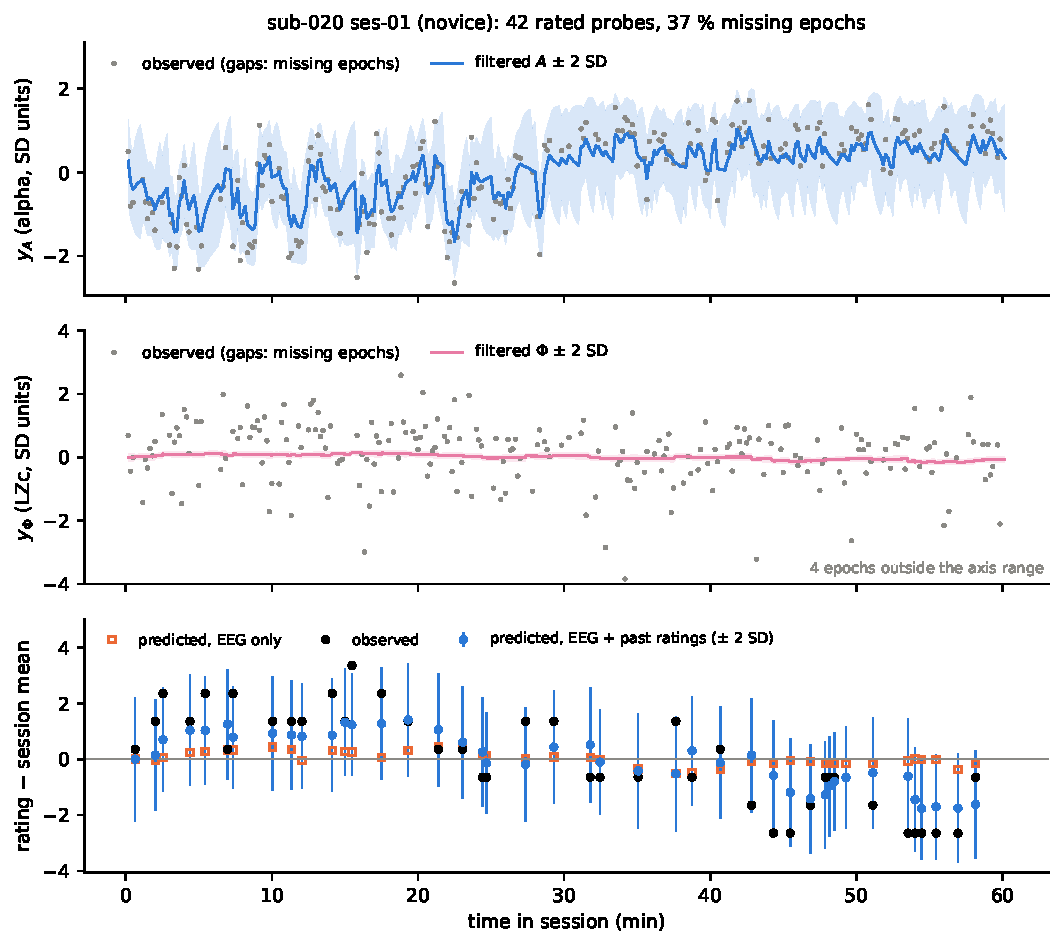
\includegraphics[width=0.49\textwidth]{fig9_realdata_session.pdf}\hfill
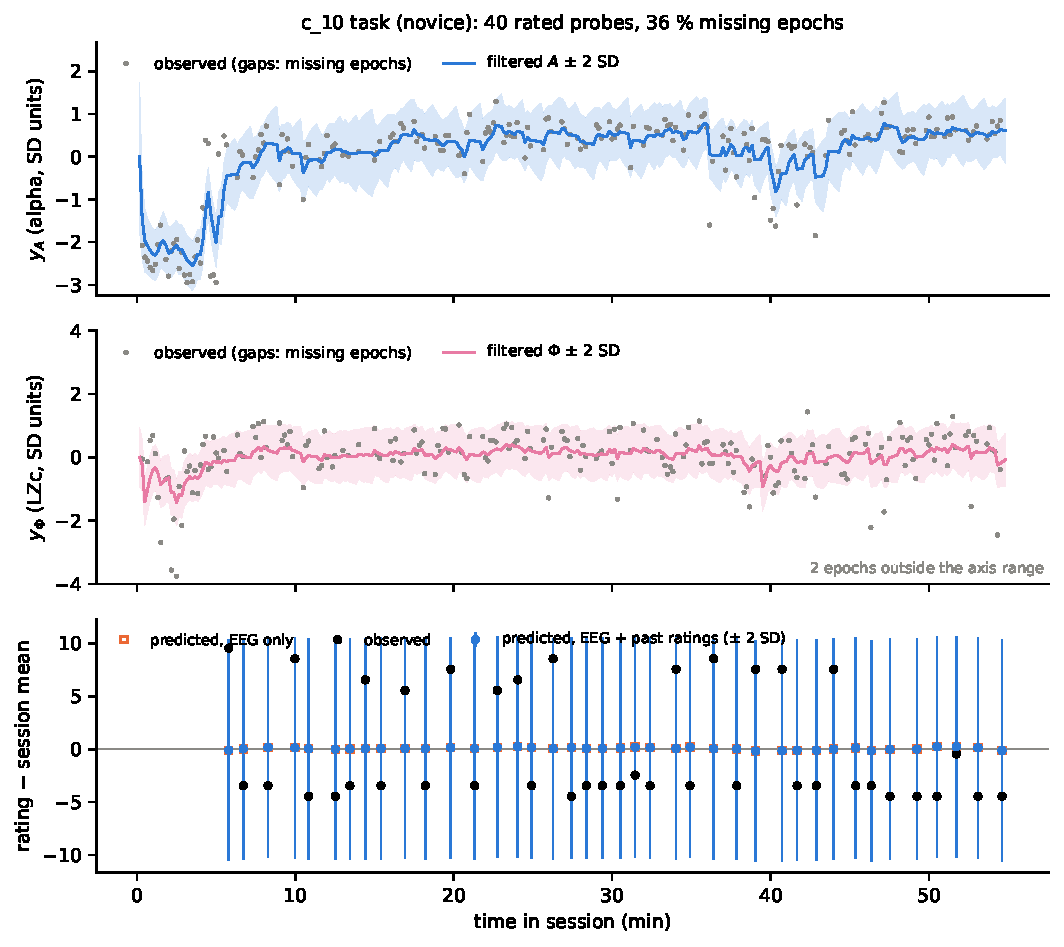
\includegraphics[width=0.49\textwidth]{fig11_osf_session.pdf}
\caption{\textbf{Một phiên được giữ của mỗi bộ dữ liệu, lọc bằng M1 tại ước lượng gộp (trong mẫu).} Trái: ds001787, sub-020 ses-01 (người mới); phải: OSF 3uszv, c\_10 (người mới); mỗi trường hợp là phiên được giữ có nhiều lần hỏi có điểm nhất. Trên: đại diện DMN $y_A$ và $A$ đã lọc $\pm2$ SD. Giữa: đại diện tích hợp $y_\Phi$ và $\Phi$ đã lọc $\pm2$ SD; trên ds001787 $\Phi$ đã lọc hầu như không động vì $y_\Phi$ gần như là nhiễu thuần, trên OSF 3uszv nó dao động theo thang vài chục giây; vài epoch ngoại lai nằm ngoài trục. Dưới: điểm tự chấm quy tâm trong phiên, với dự đoán một bước từ EEG và điểm quá khứ ($\pm2$ SD) và chỉ từ EEG. Khoảng trống là epoch thiếu. Trên OSF 3uszv đại diện alpha trôi theo thang phút, với các bước nhảy mức gần phút 5 và phút 40, và điểm luân phiên giữa khoảng $+7$ và $-5$ không có phụ thuộc chuỗi, nên mọi dự đoán nằm ở trung bình phiên.}
\label{fig:sessions}
\end{figure*}

\subsection{Sai số dự đoán và sai số đạt được (RQ1)}
Hình~\ref{fig:errors} là kết quả chính. Với bảy tham số không phụ thuộc thang của M1, nó cho thấy, trên mỗi bộ, CRB tính trước khi khoá, sai số chuẩn Fisher tại ước lượng, RMSE bootstrap và sai số chuẩn theo thông tin quan sát. Bảng~\ref{tab:errors} cho con số của hai hằng số tốc độ. Trên ds001787, cận của $\kinh$ tính trước khi xem bất kỳ EEG nào (9,1\,\%) và cận tính lại trên các phiên được giữ tại tỉ số tín hiệu trên nhiễu đo được (13,3\,\%) kẹp lấy 9,9\,\% đạt được, và bootstrap tái tạo giá trị Fisher (tỉ số 0,98). Trên OSF 3uszv, việc hỏi dày hơn và phiên dài hơn cho cận nhỏ hơn, 6,7\,\%, và sai số Fisher đạt được là 8,5\,\% với tỉ số bootstrap 1,03; tỉ số bootstrap trên Fisher là 0,98--1,69 trên ds001787 và 1,00--1,08 trên OSF 3uszv cho cả mười tham số, nên cổng E2 và F2 qua. Giả thuyết H1 được ủng hộ theo tiêu chí Fisher đã đăng ký trên cả hai bộ. Theo nghĩa Fisher, phân tích thiết kế chính xác trên ds001787 và hơi lạc quan trên OSF 3uszv, nơi sai số đạt được vượt cận tính lại trên các phiên được giữ 15\,\%; cả hai đều nằm gọn trong hệ số hai mà cận đã được kiểm chứng trên mô phỏng.

\begin{figure*}[t]
\centering
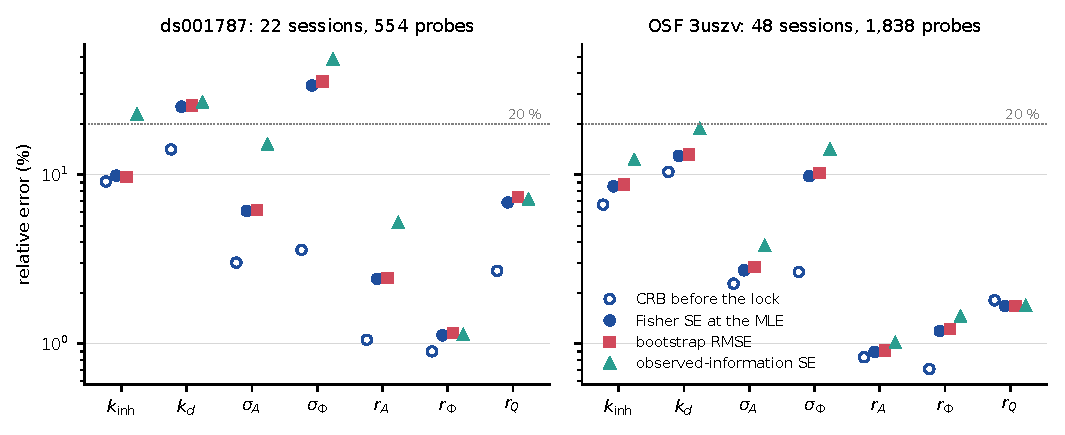
\includegraphics[width=0.95\textwidth]{fig1_pred_vs_achieved.pdf}
\caption{\textbf{Sai số tương đối dự đoán và đạt được của các tham số không phụ thuộc thang của M1 trên hai bộ dữ liệu.} Vòng tròn rỗng: cận Cramér--Rao từ thông tin Fisher chính xác tại tham số danh nghĩa trên lịch hỏi thật, tính trước mỗi lần khoá. Vòng tròn đặc: sai số chuẩn Fisher tại ước lượng hợp lý cực đại. Vuông: sai số căn quân phương của 200 lần fit lại bootstrap tham số. Tam giác: sai số chuẩn theo thông tin quan sát (Hessian số). Đường chấm là tiêu chí 20\,\% của giả thuyết H1. Với $\kinh$, ba con số đầu khớp nhau trên cả hai bộ (lớn nhất chia nhỏ nhất 1,08 và 1,32); với $\kd$, sai số Fisher vượt cận tính trước khi khoá 1,8 lần trên ds001787 và 1,2 lần trên OSF 3uszv; sai số theo thông tin quan sát của kênh công suất alpha ($\kinh$, $\sA$, $\rA$) vượt sai số Fisher 2,1--2,5 lần trên ds001787 và 1,1--1,4 lần trên OSF 3uszv.}
\label{fig:errors}
\end{figure*}

\begin{table}[t]
\caption{\textbf{Ba con số sai số cho hai hằng số tốc độ (phút$^{-1}$), là sai số tương đối tính bằng phần trăm.} CRB: trước khi khoá trên mọi thiết kế thật, trên các thiết kế được giữ, và trên các thiết kế đó với $\rA$ theo tỉ số tín hiệu trên nhiễu đo được. SE tại MLE: thông tin Fisher kỳ vọng, thông tin quan sát và hợp lý profile. RMSE: 200 lần fit lại bootstrap; tỉ số: RMSE chia SE Fisher (cổng E2/F2).}
\label{tab:errors}
\centering\scriptsize
\setlength{\tabcolsep}{2.2pt}
\begin{tabular}{llrrrrrrrrr}
\toprule
 & & & \multicolumn{3}{c}{CRB} & \multicolumn{3}{c}{SE tại MLE} & & \\
\cmidrule(lr){4-6}\cmidrule(lr){7-9}
Bộ dữ liệu & T.số & Ư.l. & khoá & giữ & SNR & Fisher & q.sát & prof. & RMSE & tỉ số \\
\midrule
ds001787  & $\kinh$ & 1,32  & 9,1  & 12,3 & 13,3 & 9,9  & 22,8 & 21,9 & 9,7  & 0,98 \\
          & $\kd$   & 0,200 & 14,1 & 19,0 & 19,1 & 25,3 & 26,7 & 26,6 & 25,7 & 1,01 \\
OSF 3uszv & $\kinh$ & 0,140 & 6,7  & 7,4  & 7,4  & 8,5  & 12,2 & 11,8 & 8,8  & 1,03 \\
          & $\kd$   & 1,58  & 10,4 & 11,5 & 11,5 & 12,9 & 18,7 & 18,3 & 13,2 & 1,02 \\
\bottomrule
\end{tabular}
\end{table}

\subsection{Dấu hiệu sai đặc tả (RQ1)}
Thông tin quan sát kể một câu chuyện khác cho kênh DMN. Trên ds001787, Hessian số cho 22,8\,\% với $\kinh$ và hợp lý profile cho 21,9\,\%, hơn gấp đôi giá trị Fisher; cùng hệ số đó, 2,1--2,5, xuất hiện với $\sA$ và $\rA$, trong khi với $\kd$, $\rPhi$ và $\rQ$ thông tin quan sát và kỳ vọng khớp nhau trong 6\,\%. Trên một bộ dữ liệu mô phỏng từ $\hat\thetav$ trên cùng 22 thiết kế, hệ số này cho $\kinh$, $\sA$ và $\rA$ là 1,05--1,07. Một khoảng cách khu trú ở một kênh và vắng mặt dưới mô hình đã fit là dấu hiệu sai đặc tả của kênh đó: công suất alpha vùng sau không được mô tả đầy đủ bởi một quá trình Ornstein--Uhlenbeck cộng nhiễu trắng. Trên OSF 3uszv dấu hiệu vẫn có nhưng yếu hơn, 1,43 với $\kinh$, 1,39 với $\sA$ và 1,13 với $\rA$ so với 0,93--0,99 trên dữ liệu mô phỏng, và không còn khu trú ở kênh alpha (1,45 với $\kd$, 1,44 với $\sPhi$); kiểm tra lặp lại R2, vốn đòi hệ số vượt 1,5, không đạt. Hình~\ref{fig:profiles} cho thấy các profile: trên ds001787 profile của $\kinh$ rộng khoảng gấp đôi đường bậc hai Fisher còn profile của $\kd$ bám theo nó; trên OSF 3uszv profile của $\kinh$ và $\kd$ rộng gấp 1,4 lần đường bậc hai, và profile của $\kappa$ bất đối xứng. Theo tiêu chí dựa trên hàm hợp lý, H1 vì thế không được ủng hộ trên ds001787 (21,9\,\%, vừa vượt 20\,\%) và được ủng hộ trên OSF 3uszv (11,8\,\%). Chúng tôi báo cáo khoảng profile làm độ bất định của $\kinh$ xuyên suốt.

\begin{figure*}[t]
\centering
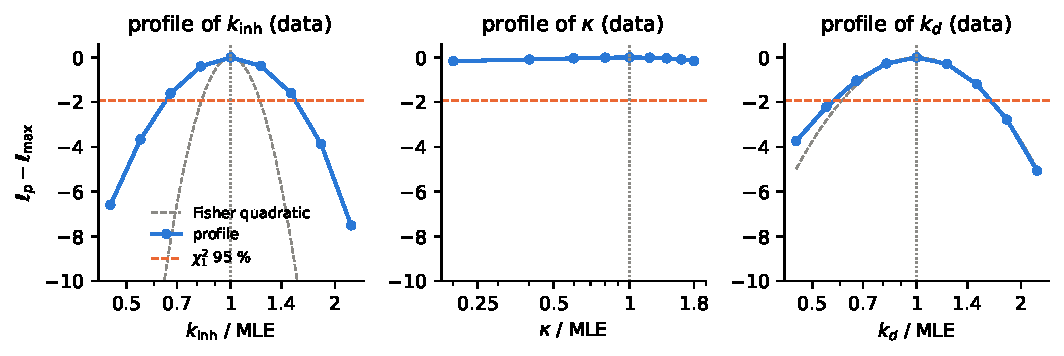
\includegraphics[width=0.82\textwidth]{fig10_realdata_profiles.pdf}\\[3pt]
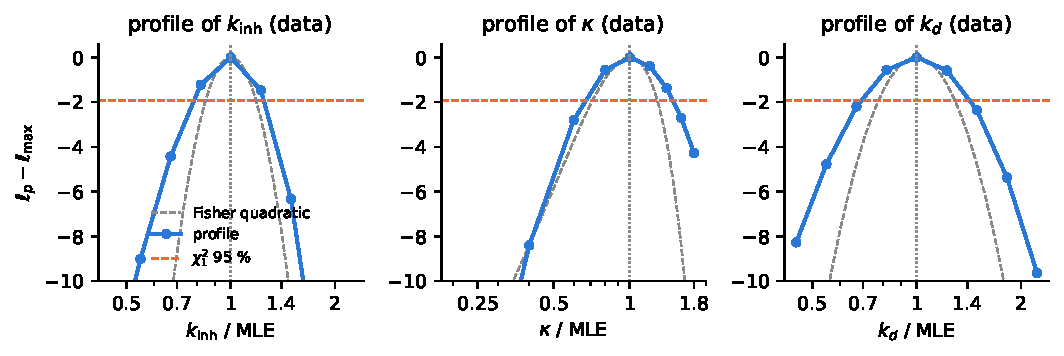
\includegraphics[width=0.82\textwidth]{fig12_osf_profiles.pdf}
\caption{\textbf{Log-hợp lý profile của ba hằng số tốc độ, mọi tham số khác được tối ưu lại tại mỗi điểm.} Trên: ds001787; dưới: OSF 3uszv. Nét đứt xám: xấp xỉ bậc hai suy từ thông tin Fisher kỳ vọng tại ước lượng hợp lý cực đại; cam: ngưỡng 95\,\% của $\chi^2_1$. Trên ds001787 profile của $\kinh$ rộng khoảng gấp đôi đường bậc hai (khoảng 95\,\% là 0,86--2,02~phút$^{-1}$), profile của $\kd$ bám theo nó, và profile của $\kappa$ phẳng vì $\hat\kappa\approx0$. Trên OSF 3uszv profile của $\kinh$ rộng gấp 1,38 lần đường bậc hai (0,110--0,175~phút$^{-1}$), của $\kd$ gấp 1,4 lần, và profile của $\kappa$, vốn âm, bất đối xứng (từ $-0{,}50$ đến $-0{,}23$).}
\label{fig:profiles}
\end{figure*}

\subsection{Ước lượng}
Bảng~\ref{tab:compare} đặt hai fit cạnh nhau. Trên ds001787 đại diện DMN hồi phục nhanh, $1/\hat k_{\mathrm{inh}}=0{,}76$~phút (khoảng profile 0,49--1,17~phút), so với 5~phút danh nghĩa của phân tích thiết kế, còn biến tích hợp ẩn chậm, $1/\hat k_d=5{,}0$~phút (3,1--8,7~phút); hệ số ghép $\kappa$ không phân biệt được với 0. Trên OSF 3uszv đại diện DMN chậm, $1/\hat k_{\mathrm{inh}}=7{,}1$~phút (5,7--9,1~phút), gấp chín lần giá trị của ds001787, còn biến tích hợp nhanh, $1/\hat k_d=0{,}63$~phút (0,45--0,91~phút), nhanh gấp tám lần trước: hai hằng số thời gian đã đổi chỗ cho nhau, và R1 trượt chín lần. Hệ số ghép nay xác định được và âm, $\hat\kappa=-0{,}33$ (từ $-0{,}50$ đến $-0{,}23$). Chất lượng các đại diện khác nhau giữa hai bộ. Trên ds001787 kênh DMN có tỉ số tín hiệu trên nhiễu 1,11 so với 1,58 danh nghĩa và kênh tích hợp 0,06 so với 2,4 danh nghĩa: thước đo độ phức tạp đã kiểm soát phổ hầu như không mang tín hiệu chậm. Trên OSF 3uszv kênh DMN đạt tỉ số danh nghĩa (1,57) và kênh tích hợp 0,54, gấp tám lần giá trị trên ds001787.

\begin{table*}[t]
\caption{\textbf{Hai fit đã đăng ký trước đặt cạnh nhau.} Hằng số thời gian tính bằng phút với khoảng profile 95\,\%; hệ số khuếch đại với khoảng Fisher 95\,\% và theo đơn vị SD trong phiên của điểm tự chấm (1,11 và 5,22). SE của $\kinh$: CRB trước khi khoá, Fisher, thông tin quan sát, hợp lý profile. Q.sát/kỳ vọng: SE theo thông tin quan sát chia SE theo thông tin kỳ vọng trên dữ liệu thật (trong ngoặc: trên dữ liệu mô phỏng từ fit). \mbox{\mathversion{normal}$\Delta$}LPD: mật độ dự đoán log ngoài mẫu của M1 trừ N2 (chỉ EEG) và trừ N1 (EEG và điểm quá khứ). Hiệu nhóm: $\log\kinh$, fit người lâu năm trừ fit người mới, khoảng Wald 95\,\%. Phân tích gộp: $1/\kinh$ hiệu ứng ngẫu nhiên trên những người có SE hữu hạn và SD giữa người $\tau$ của $\log\kinh$. Độ nhạy: số biến thể đã khoá giữ nguyên dấu của $\alpha$, dấu của $\beta$ và khoảng profile của $1/\kinh$.}
\label{tab:compare}
\centering\footnotesize
\setlength{\tabcolsep}{4pt}
\begin{tabular}{lll}
\toprule
 & ds001787 & OSF 3uszv \\
\midrule
Phiên giữ / ghi; số người                & 22 / 40; 16 & 48 / 58; 48 \\
Lần hỏi có điểm; khoảng hỏi; phiên      & 554; 1,6~phút; 45~phút & 1\,838; 77~s; 57~phút \\
Thang điểm; SD trong phiên               & $-3$ đến $3$; 1,11 & $-7$ đến $7$; 5,22 \\
$1/\kinh$ (phút)                         & 0,76 [0,49; 1,17] & 7,1 [5,7; 9,1] \\
$1/\kd$ (phút)                           & 5,0 [3,1; 8,7] & 0,63 [0,45; 0,91] \\
$\kappa$                                 & $\approx0$, profile phẳng & $-0{,}33$ [$-0{,}50$; $-0{,}23$] \\
SNR của $y_A$; của $y_\Phi$              & 1,11; 0,06 & 1,57; 0,54 \\
SE của $\kinh$: CRB / Fisher / q.\,sát / profile & 9,1 / 9,9 / 22,8 / 21,9\,\% & 6,7 / 8,5 / 12,2 / 11,8\,\% \\
RMSE bootstrap / SE Fisher của $\kinh$   & 0,98 & 1,03 \\
SE q.\,sát/kỳ vọng: $\kinh$, $\sA$, $\rA$ & 2,30; 2,48; 2,14 (1,05--1,07) & 1,43; 1,39; 1,13 (0,93--0,99) \\
$\alpha$ [95\,\%]; theo SD điểm          & 13,1 [4,9; 21,3]; 11,8 & 0,79 [$-0{,}24$; 1,82]; 0,15 \\
$\beta$ [95\,\%]; theo SD điểm           & $-0{,}03$ [$-0{,}19$; $0{,}13$]; $-0{,}02$ & 0,02 [$-0{,}34$; $0{,}38$]; 0,00 \\
$\Delta$LPD so với N2; so với N1         & $-0{,}010$; $-0{,}031$ & $+0{,}000$; $-0{,}001$ \\
Tự tương quan trễ 1 của điểm tự chấm     & 0,22 & $-0{,}01$ \\
Hiệu nhóm của $\log\kinh$                & $-1{,}19$ [$-1{,}56$; $-0{,}81$] & $+0{,}14$ [$-0{,}20$; $0{,}47$] \\
Phân tích gộp: $1/\kinh$; $\tau$; số người & 0,95 [0,40; 2,26]; 1,19; 9 & 3,3 [2,0; 5,7]; 1,49; 35 \\
Trung vị p Ljung--Box: $y_A$, $y_\Phi$   & 0,27; 0,40 & 0,06; 0,42 \\
Độ nhạy: $\alpha$, $\beta$, $1/\kinh$ giữ nguyên & 6/6; 4/6; 4/6 & 5/6; 1/6; 4/6 \\
Cổng                                     & E0--E3 qua & F0--F3 qua \\
\bottomrule
\end{tabular}
\end{table*}

\subsection{Hệ số khuếch đại và dự đoán ngoài mẫu (RQ2)}
Trên ds001787 hệ số khuếch đại từ biến tích hợp sang điểm là dương, $\hat\alpha=13{,}1$ (khoảng Fisher 95\,\% 4,9--21,3; không lần bootstrap nào ra giá trị không dương), như giả thuyết H3 dự đoán. Ý nghĩa của nó hạn chế: vì $y_\Phi$ thực chất là nhiễu, $\Phi$ ẩn được xác định hầu như hoàn toàn bởi chính điểm tự chấm, $\alpha$ và $\sPhi$ đánh đổi cho nhau (tương quan bootstrap giữa $\log\sPhi$ và $\alpha$: $-0{,}83$), và chỉ đóng góp của $\Phi$ vào phương sai điểm là xác định tốt. Trên OSF 3uszv, nơi $\Phi$ bị kênh độ phức tạp ghim lại, $\hat\alpha=0{,}79$ với khoảng chứa 0 (từ $-0{,}24$ đến $1{,}82$; 11 trong 200 lần bootstrap ra giá trị không dương): H3 không được ủng hộ. Theo đơn vị SD trong phiên của điểm, hệ số này là 11,8 trên ds001787 và 0,15 trên OSF 3uszv. Hệ số DMN là $\hat\beta=-0{,}03$ (từ $-0{,}19$ đến $0{,}13$) và $0{,}02$ (từ $-0{,}34$ đến $0{,}38$): dấu mà H4 hỏi không xác định được ở bộ nào, và công suất alpha vùng sau không đóng góp phát hiện được vào điểm.

Bảng~\ref{tab:loso} cho so sánh bỏ-một-phiên của giả thuyết H2. Trên ds001787, chỉ với EEG, M1 dự đoán điểm không tốt hơn hồi quy tức thời N2; với EEG và điểm quá khứ nó thắng trung bình chạy N3 nhưng không thắng mô hình chỉ có điểm N1, mô hình có mật độ dự đoán log tốt nhất và sai số nhỏ nhất trong mọi mô hình. Ưu thế so với N3 vì thế đến từ phụ thuộc chuỗi của báo cáo (tự tương quan trễ 1 là 0,22), không phải từ EEG. Trên OSF 3uszv, M1 không phân biệt được với N2 và N1 ($\Delta\mathrm{LPD}$ là $+0{,}0004$ và $-0{,}0006$), với sai số tuyệt đối trung bình 4,5--4,6 trên thang 14 mức cho mọi mô hình trừ trung bình chạy (4,7), và vì một lý do căn bản hơn: điểm của bộ này không có phụ thuộc chuỗi để mà dự đoán (tự tương quan trễ 1 là $-0{,}01$), nên điểm quá khứ cũng không giúp gì, và phân phối hai cực của chúng nằm ngoài tầm với của một hàm đọc ra Gauss (Phụ lục~\ref{app:ppc}). H2 không được ủng hộ ở bộ nào.

\begin{table*}[t]
\caption{\textbf{Dự đoán bỏ-một-phiên cho điểm tự chấm (giả thuyết H2), (a) chỉ từ EEG và (b) từ EEG và điểm quá khứ.} LPD: mật độ dự đoán log Gauss trung bình mỗi lần hỏi; MAE: sai số tuyệt đối trung bình. \mbox{\mathversion{normal}$\Delta$}LPD: M1 trừ mô hình rỗng với khoảng bootstrap 95\,\% theo phiên. N2: hồi quy tức thời lên $(y_A,y_\Phi)$; N1: M1 chỉ với kênh điểm; N3: trung bình chạy của điểm quá khứ.}
\label{tab:loso}
\centering\footnotesize
\setlength{\tabcolsep}{5pt}
\begin{tabular}{llrrrrr}
\toprule
 & So sánh & LPD M1 & LPD rỗng & $\Delta$LPD [95\,\%] & MAE M1 & MAE rỗng \\
\midrule
ds001787 & (a) với N2 & $-1{,}546$ & $-1{,}541$ & $-0{,}010$ [$-0{,}039$; $0{,}017$] & 0,93 & 0,92 \\
(554 lần hỏi) & (b) với N1 & $-1{,}472$ & $-1{,}421$ & $-0{,}031$ [$-0{,}103$; $0{,}009$] & 0,88 & 0,84 \\
 & (b) với N3 & $-1{,}472$ & $-1{,}626$ & $+0{,}154$ [$0{,}083$; $0{,}233$] & 0,88 & 1,00 \\
\midrule
OSF 3uszv & (a) với N2 & $-3{,}0746$ & $-3{,}0749$ & $+0{,}0004$ [$-0{,}0006$; $0{,}0014$] & 4,54 & 4,56 \\
(1\,838 lần hỏi) & (b) với N1 & $-3{,}0746$ & $-3{,}0740$ & $-0{,}0006$ [$-0{,}0018$; $0{,}0006$] & 4,54 & 4,55 \\
 & (b) với N3 & $-3{,}0746$ & $-3{,}1445$ & $+0{,}0712$ [$0{,}0609$; $0{,}0815$] & 4,54 & 4,66 \\
\bottomrule
\end{tabular}
\end{table*}

\subsection{Nhóm và từng người}
Trên ds001787, khi fit riêng, nhóm lâu năm có $\kinh$ nhỏ hơn nhóm mới (hiệu log $-1{,}19$, khoảng Wald 95\,\% từ $-1{,}56$ đến $-0{,}81$), ngược với giả thuyết H5. Hai fit riêng khác nhau chủ yếu ở cách chia phương sai công suất alpha giữa trạng thái và nhiễu quan sát (tỉ số tín hiệu trên nhiễu 1,05 so với 2,23), và $\kinh$ đánh đổi với cách chia đó: khi mọi tham số khác dùng chung, hiệu log co về $-0{,}18$ và kiểm định một bậc tự do đã đăng ký không có ý nghĩa ($\chi^2_1=3{,}3$, $p=0{,}068$), dù hai nhóm có khác nhau ở tham số nào đó ($\chi^2_{10}=41$). Hai nhóm còn khác nhau về giới và tuổi (10 trong 12 so với 2 trong 12 là nam, tuổi trung bình 39 so với 48). Trên OSF 3uszv, với 25 và 23 phiên, hai fit theo nhóm cho $\hat k_{\mathrm{inh}}=0{,}154$ và $0{,}134~\text{phút}^{-1}$, hiệu log $+0{,}14$ (từ $-0{,}20$ đến $0{,}47$; $\chi^2_1=2{,}67$, $p=0{,}10$), dưới khác biệt nhỏ nhất phát hiện được 0,37: cả F-H5a lẫn F-H5b đều không được ủng hộ, và hiệu thấy trên ds001787 không lặp lại. Hai nhóm khác nhau ở các tham số khác ($\chi^2_{10}=256$): ở người mới, biến tích hợp nhanh và ồn ($1/\kd=0{,}33$~phút, $\sPhi=1{,}1$) và gắn dương với báo cáo ($\alpha=2{,}0$, $\beta=+0{,}75$); ở người lâu năm nó chậm hơn ($1/\kd=0{,}89$~phút, $\sPhi=0{,}68$) và cả hai hệ số khuếch đại gần không hoặc âm ($\alpha=-0{,}15$, $\beta=-0{,}66$). Fit theo từng người cho sai số chuẩn hữu hạn ở 9 trong 16 người trên ds001787 và 35 trong 48 trên OSF 3uszv (ở phần lớn số còn lại $\sPhi$ được ước lượng bằng 0). Phân tích gộp của họ cho hằng số thời gian DMN 0,95~phút (0,40--2,26) và 3,3~phút (2,0--5,7) với độ lệch chuẩn giữa người của $\log\kinh$ là 1,19 và 1,49 đơn vị log ($I^2=0{,}92$ ở cả hai): các fit gộp cùng lắm mô tả một người tập trung bình.

\subsection{Kiểm tra mô hình và độ nhạy}
Innovation gần trắng trên ds001787 (trung vị p Ljung--Box $0{,}27$ cho $y_A$ và $0{,}40$ cho $y_\Phi$; bốn trong 22 phiên dưới 0,01 với $y_A$) và kém hơn trên OSF 3uszv ($p=0{,}058$ cho $y_A$, với 17 trong 48 phiên dưới 0,01; $0{,}42$ cho $y_\Phi$); innovation của hai kênh không tương quan ở cả hai (trung vị 0,05), nên ma trận nhiễu quan sát chéo được giữ. Kiểm tra dự đoán hậu nghiệm (Phụ lục~\ref{app:ppc}) tái tạo được phụ thuộc chuỗi của điểm trên ds001787 (tự tương quan trễ 1 là 0,22, mô phỏng 0,26, dải 0,15--0,37) và việc không có phụ thuộc chuỗi trên OSF 3uszv ($-0{,}01$; mô phỏng $-0{,}03$, dải từ $-0{,}08$ đến $0{,}02$), nhưng không tái tạo được phần giữa lệch của phân phối ds001787 lẫn phân phối hai cực của OSF, và trên cả hai bộ người lâu năm chấm điểm với độ phân tán nhỏ hơn mức mô hình gộp ngụ ý (OSF: hiệu SD trong phiên quan sát $-1{,}01$, mô phỏng $-0{,}31$, dải từ $-0{,}55$ đến $-0{,}05$).

Bảng~\ref{tab:sens} liệt kê các phân tích độ nhạy. Trên ds001787 $\alpha$ giữ dương ở cả sáu biến thể đã khoá, dấu của $\beta$ giữ ở bốn, và $1/\kinh$ nằm trong khoảng profile ở bốn: đại diện theta trán cho 4,0~phút, và biến thể chỉ giữ phiên có không quá 20\,\% epoch thiếu giữ hai phiên và suy biến. Trên OSF 3uszv biến thể đó không giữ phiên nào, vì riêng cửa sổ hỏi đã vượt 20\,\% ở mọi phiên, một sơ suất của bản đăng ký, nên sáu biến thể chạy được; dấu của $\alpha$ giữ ở năm (nó âm với đại diện số mũ aperiodic), dấu của $\beta$ ở một, và $1/\kinh$ nằm trong khoảng ở bốn (theta trán cho 17~phút và z-score theo phiên 4,8~phút). Quy tắc 80\,\% vì thế đạt với dấu của $\alpha$ trên cả hai bộ và không với gì khác, và các ước lượng được trình bày theo lối mô tả. Một biến thể ngoài đăng ký trên OSF 3uszv, thêm sau khi xem Hình~\ref{fig:sessions}, che EEG trước lần hỏi đầu tiên (các phiên mở đầu bằng hướng dẫn và một lần hỏi tập dượt, tiếng chuông đầu tiên đến sau trung bình 6,8~phút): hằng số thời gian DMN tăng từ 7,1 lên 16~phút, nên bước chuyển mức alpha ở đầu phiên là phần nhanh nhất của đại diện này.

\begin{table*}[t]
\caption{\textbf{Phân tích độ nhạy: ước lượng gộp, hằng số thời gian tính bằng phút.} Quy tắc cố định 150~$\mu$V là quy tắc chính đã khoá của ds001787 và một biến thể đã khoá của OSF 3uszv; quy tắc thích ứng là biến thể ngoài đăng ký của ds001787 và quy tắc chính đã khoá của OSF 3uszv. Dòng cuối là biến thể ngoài đăng ký và không tính vào quy tắc độ bền. Trên ds001787 biến thể không quá 20\,\% epoch thiếu giữ hai phiên và suy biến; trên OSF 3uszv nó không giữ phiên nào.}
\label{tab:sens}
\centering\footnotesize
\setlength{\tabcolsep}{5pt}
\begin{tabular}{lrrrrrrrr}
\toprule
 & \multicolumn{4}{c}{ds001787} & \multicolumn{4}{c}{OSF 3uszv} \\
\cmidrule(lr){2-5}\cmidrule(lr){6-9}
Biến thể & $n$ & $\alpha$ & $\beta$ & $1/\kinh$ & $n$ & $\alpha$ & $\beta$ & $1/\kinh$ \\
\midrule
Phân tích chính                      & 22 & 13,10 & $-0{,}026$ & 0,76 & 48 & 0,79 & $+0{,}018$ & 7,12 \\
$y_A$: alpha tuần hoàn               & 22 & 13,10 & $-0{,}069$ & 0,52 & 48 & 0,79 & $+0{,}069$ & 7,74 \\
$y_A$: theta trán                    & 22 & 13,08 & $-0{,}389$ & 3,98 & 48 & 0,76 & $-0{,}293$ & 16,76 \\
$y_\Phi$: số mũ aperiodic đổi dấu    & 22 & 13,08 & $+0{,}045$ & 0,76 & 48 & $-0{,}10$ & $-0{,}127$ & 7,91 \\
z-score theo phiên                   & 22 & 13,10 & $-0{,}051$ & 0,90 & 48 & 0,82 & $-0{,}108$ & 4,81 \\
Không quá 20\,\% epoch thiếu         &  2 & 399,6 & $-0{,}239$ & 0,23 &  0 & -- & -- & -- \\
20 lần hỏi đầu                       & 22 & 13,09 & $+0{,}096$ & 0,76 & 48 & 1,43 & $-0{,}096$ & 7,10 \\
Quy tắc cố định 150~$\mu$V           & \multicolumn{4}{c}{(chính)} & 24 & 0,36 & $-0{,}470$ & 5,74 \\
Quy tắc thích ứng                    & 39 & 0,97 & $+0{,}215$ & 0,48 & \multicolumn{4}{c}{(chính)} \\
Che EEG trước lần hỏi đầu            & -- & -- & -- & -- & 48 & 1,02 & $+0{,}285$ & 16,00 \\
\bottomrule
\end{tabular}
\end{table*}

\subsection{So sánh với tham số của BQI (RQ3)}
\label{sec:res-bqi}
Bảng~\ref{tab:bqi} đặt các ước lượng cạnh các dự đoán T1--T5 của BQI (Mục~\ref{sec:theory-pred}) và các giá trị mà BQI fit từ dữ liệu phân tích gộp \cite[Bảng~5]{BQI}. Hằng số thời gian không phụ thuộc thang nên so trực tiếp được; hệ số ghép và các hệ số khuếch đại phụ thuộc đơn vị của các đại diện đã chuẩn hoá và của thang điểm, nên chỉ so được dấu. Không bộ nào tái tạo được các hằng số thời gian của BQI: hằng số thời gian DMN là 0,76 và 7,1~phút so với 23~phút, hằng số thời gian tích hợp là 5,0 và 0,63~phút so với 29~phút, và giá trị BQI nằm ngoài cả bốn khoảng profile. Hệ số ghép, dương trong \cite[pt.~(53)]{BQI}, không phân biệt được với 0 trên ds001787 và âm trên OSF 3uszv. Hệ số $\alpha$ dương ở cả hai bộ như trong BQI, nhưng khoảng tin cậy chỉ loại 0 trên ds001787; dấu của $\beta$, dương trong BQI, không xác định được ở bộ nào; và khác biệt nhóm suy ra từ \cite[pt.~(51) và Mục~7.5]{BQI} bị đảo chiều trên ds001787 và vắng mặt trên OSF 3uszv. Trong năm dự đoán, chỉ T3 được tái tạo về dấu, và chỉ xác định được dấu trên ds001787.

\begin{table*}[t]
\caption{\textbf{Giá trị tham số của BQI và các ước lượng trên hai bộ dữ liệu.} BQI: fit bình phương tối thiểu từ dữ liệu phân tích gộp \cite[Bảng~5]{BQI}. Hằng số thời gian tính bằng phút với khoảng profile 95\,\%; $\kappa$ với khoảng profile; hệ số khuếch đại với khoảng Fisher 95\,\%; hiệu nhóm của $\log\kinh$ (lâu năm trừ mới) với khoảng Wald. Hệ số ghép và hệ số khuếch đại tính theo đơn vị của các đại diện và điểm đã chuẩn hoá, nên chỉ so được dấu với BQI.}
\label{tab:bqi}
\centering\footnotesize
\setlength{\tabcolsep}{5pt}
\begin{tabular}{llll}
\toprule
Đại lượng & BQI & ds001787 & OSF 3uszv \\
\midrule
$1/\kinh$ (phút) & 23 & 0,76 [0,49; 1,17] & 7,1 [5,7; 9,1] \\
$1/\kd$ (phút) & 29 & 5,0 [3,1; 8,7] & 0,63 [0,45; 0,91] \\
Dấu của $\kappa$ & $+$ & $\approx0$, profile phẳng & $-$ ($-0{,}33$ [$-0{,}50$; $-0{,}23$]) \\
Dấu của $\alpha$ & $+$ (2,34) & $+$ (13,1 [4,9; 21,3]) & $+$, chưa xác định (0,79 [$-0{,}24$; 1,82]) \\
Dấu của $\beta$ & $+$ (1,87) & chưa xác định & chưa xác định \\
Lâu năm $-$ mới, $\log\kinh$ & $>0$ & $-1{,}19$ [$-1{,}56$; $-0{,}81$] & $+0{,}14$ [$-0{,}20$; 0,47] \\
\bottomrule
\end{tabular}
\end{table*}

\subsection{Điều gì lặp lại (RQ4)}
Bảng~\ref{tab:tests} liệt kê mọi giả thuyết và kiểm tra đã đăng ký cùng kết cục. Ba kết quả chung cho hai bộ và hai kết quả thì không. (i) Các con số sai số theo Fisher chính xác trên cả hai: với $\kinh$, cận tính trước khi khoá, SE Fisher tại ước lượng và RMSE bootstrap chênh nhau nhiều nhất 8\,\% trên ds001787 và 32\,\% trên OSF 3uszv, và trên cả hai SE dựa trên hàm hợp lý của kênh alpha vượt SE Fisher. (ii) Không đại diện EEG nào cải thiện dự đoán ngoài mẫu cho báo cáo ở bộ nào. (iii) Độ dị biệt giữa người của $\log\kinh$ lớn ở cả hai ($\tau$ là 1,2 và 1,5). (iv) $\alpha>0$ không lặp lại: ước lượng dương ở cả hai, nhưng khoảng tin cậy chỉ loại 0 trên ds001787, và ở cả hai giá trị của nó theo SD của điểm nói lên ít điều. (v) Bản thân các hằng số tốc độ không lặp lại: $1/\kinh$ là 0,76~phút trên ds001787 và 7,1~phút trên OSF 3uszv, $1/\kd$ là 5,0 so với 0,63~phút, và chiều của khác biệt nhóm khác nhau.

\begin{table*}[t]
\caption{\textbf{Các giả thuyết đã đăng ký và kiểm tra lặp lại cùng kết cục trên hai bộ dữ liệu (khoảng là 95\,\%).}}
\label{tab:tests}
\centering\scriptsize
\setlength{\tabcolsep}{3pt}
\begin{tabular}{lll}
\toprule
Giả thuyết & ds001787 & OSF 3uszv \\
\midrule
H1: SE của $\kinh$ không quá 20\,\% & Fisher 9,9\,\% (profile 21,9\,\%): ủng hộ (Fisher) & Fisher 8,5\,\% (profile 11,8\,\%): ủng hộ \\
H2: M1 thắng các mô hình rỗng & $\Delta$LPD $-0{,}010$ (N2), $-0{,}031$ (N1): không ủng hộ & $+0{,}0004$ (N2), $-0{,}0006$ (N1): không ủng hộ \\
H3: $\alpha>0$ & 13,1 [4,9; 21,3]: ủng hộ & 0,79 [$-0{,}24$; 1,82]: không ủng hộ \\
H4: dấu của $\beta$ & $-0{,}03$ [$-0{,}19$; 0,13]: không xác định & 0,02 [$-0{,}34$; 0,38]: không xác định \\
H5: $\kinh$ cao hơn ở người lâu năm & $-1{,}19$ [$-1{,}56$; $-0{,}81$]; LR $p=0{,}068$: không ủng hộ & $+0{,}14$ [$-0{,}20$; 0,47]; LR $p=0{,}10$: không ủng hộ (a, b) \\
R1: $1/\kinh$ trong 0,49--1,17 phút & -- & 7,1 phút [5,7; 9,1]: không lặp lại \\
R2: SE q.sát/kỳ vọng $>1{,}5$, $\approx1$ khi mô phỏng & 2,30; 1,05 & 1,43; 0,93: không lặp lại \\
R3: $1/\kd$ & 5,0 phút [3,1; 8,7] & 0,63 phút [0,45; 0,91] \\
\bottomrule
\end{tabular}
\end{table*}

\subsection{Vì sao hằng số thời gian khác nhau: một mô phỏng}
Việc hai hằng số thời gian đổi chỗ có một cách đọc đơn giản. Trên ds001787, đại diện độ phức tạp là nhiễu, nên $\Phi$ và $\kd$ được xác định bởi điểm tự chấm và $1/\kd$ đo sự trôi chậm của báo cáo; trên OSF 3uszv đại diện độ phức tạp mang tín hiệu 40~s ghim $\Phi$ lại, báo cáo không trôi, còn đại diện alpha trôi theo thang phút trong các phiên dài một giờ (Hình~\ref{fig:sessions}). Hình~\ref{fig:sim} cho thấy fit Ornstein--Uhlenbeck làm gì với một đặc trưng như vậy. Khi đặc trưng là tổng của một thành phần nhanh (0,5~phút) và một thành phần chậm (3, 7 hoặc 15~phút), hằng số thời gian fit được dịch đơn điệu từ giá trị nhanh sang giá trị chậm khi tỉ trọng phương sai của thành phần chậm tăng: với tỉ trọng bằng nhau fit trả về 1,2; 1,7 và 1,9~phút, và giá trị chậm chỉ đạt được khi thành phần chậm chiếm gần hết phương sai (ở tỉ trọng 0,8, thành phần 7~phút cho 3,6~phút và thành phần 15~phút cho 7,5~phút). Một hằng số tốc độ duy nhất ước lượng từ một đặc trưng chưa hiệu chuẩn vì thế là tổng hợp có trọng số phương sai của mọi thang thời gian mà đặc trưng đó chứa trong bản ghi đó, phụ thuộc vào montage, độ dài phiên và phương pháp tập; đại diện theta trán cho 4~phút trên bộ này và 17~phút trên bộ kia cũng vì lý do đó. Hằng số thời gian DMN của M1 là tính chất của đặc trưng, chưa phải của một quá trình DMN.

\begin{figure}[t]
\centering
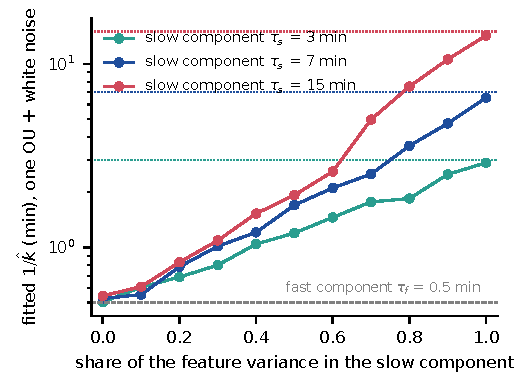
\includegraphics[width=\columnwidth]{fig2_ou_timescale.pdf}
\caption{\textbf{Fit Ornstein--Uhlenbeck trả về thang thời gian trội của đặc trưng được đưa vào.} Đặc trưng mô phỏng là tổng của một thành phần nhanh ($\tau_f=0{,}5$~phút), một thành phần chậm ($\tau_s$ bằng 3, 7 hoặc 15~phút, đường chấm) và nhiễu trắng, trên thiết kế của OSF 3uszv (48 phiên 57~phút với cửa sổ hỏi và thêm 10\,\% epoch thiếu). Nó được fit bằng một quá trình Ornstein--Uhlenbeck cộng nhiễu trắng, tức kênh DMN của M1. Hằng số thời gian fit được dịch từ $\tau_f$ sang $\tau_s$ khi tỉ trọng phương sai của thành phần chậm tăng.}
\label{fig:sim}
\end{figure}

%% VI. Thảo luận: diễn giải theo câu hỏi nghiên cứu, hàm ý, hạn chế. Được access_vi.tex \input.
\section{Thảo luận}
\label{sec:discussion}

\subsection{Phân tích thiết kế đã đúng ở đâu (RQ1)}
Bài đồng hành hứa rằng thông tin Fisher chính xác của M1 có thể dùng để lên kế hoạch một nghiên cứu lấy mẫu trải nghiệm. Trên hai thiết kế thật, với lịch hỏi không đều, một phần ba epoch thiếu và các phiên bị loại bởi quy tắc nhiễu giả, cận tính trước khi khoá, sai số chuẩn Fisher tại ước lượng và sai số bootstrap của $\kinh$ chênh nhau nhiều nhất 8\,\% trên ds001787 và 32\,\% trên OSF 3uszv. Trên ds001787, 9,9\,\% đạt được nằm giữa cận tính trước khi khoá và cận tính lại tại tỉ số tín hiệu trên nhiễu đo được (9,1--13,3\,\%); trên OSF 3uszv, 8,5\,\% đạt được vượt cận tính lại (7,4\,\%) 15\,\%. Với $\kd$, cận tính trước khi khoá lạc quan 1,8 lần và 1,2 lần. Thứ tự giữa hai bộ cũng được dự đoán: hỏi dày hơn và phiên dài hơn của OSF 3uszv cho cận nhỏ hơn và sai số đạt được nhỏ hơn. Một phân tích thiết kế kiểu này vì thế dùng được cho mục đích của nó, quyết định cần bao nhiêu người, phiên dài bao nhiêu và hỏi bao nhiêu lần, miễn là sai số nó nêu được hiểu là sai số Fisher của một mô hình được giả định là đúng.

\subsection{Điều nó không lường trước được (RQ1)}
Một cận không lường trước được sai đặc tả, và kênh công suất alpha sai đặc tả trên cả hai bộ: sai số theo thông tin quan sát và theo profile của $\kinh$, $\sA$ và $\rA$ vượt sai số Fisher 2,1--2,5 lần trên ds001787 và 1,1--1,4 lần trên OSF 3uszv, và phần vượt biến mất trên dữ liệu mô phỏng từ fit. Phép chẩn đoán này rẻ, vì chỉ cần một Hessian và một bộ dữ liệu mô phỏng, và chúng tôi khuyến nghị dùng nó bên cạnh bootstrap, vốn không nhìn thấy sai đặc tả vì mô phỏng từ chính mô hình. Trong thực hành, các con số của bản đồ thiết kế nên được đọc như cận dưới mỗi khi một đại diện chưa chắc tuân theo mô hình, và khoảng dựa trên hàm hợp lý nên được báo cáo bên cạnh khoảng Fisher; trên ds001787 hai tiêu chí cho H1 cho kết luận khác nhau.

\subsection{Mô hình quan sát là nút thắt (RQ2)}
Hai đại diện chúng tôi đăng ký không mang thông tin phát hiện được về báo cáo ngoài phụ thuộc chuỗi của chính báo cáo, ở bộ nào cũng vậy. Kênh độ phức tạp là nhiễu trên ds001787 và, trên OSF 3uszv, là một tín hiệu 40~s không liên quan đến báo cáo; alpha vùng sau không gắn với điểm ở bộ nào. Động lực của M1 xác định được và được ước lượng với độ chính xác đã dự đoán, nhưng hàm đọc ra từ đặc trưng EEG sang trạng thái được báo cáo mới là nơi thiếu thông tin. Điều này phù hợp với quan hệ gián tiếp giữa alpha vùng sau và DMN mà các nghiên cứu ghi đồng thời EEG--fMRI tìm thấy \cite{Laufs2003,Mantini2007}. Tìm một đặc trưng EEG bám theo trạng thái được báo cáo, với tỉ số tín hiệu trên nhiễu trong dải mà phân tích thiết kế cho thấy là cần thiết, là bài toán mở mà lớp mô hình này để lại cho người làm thực nghiệm, và các bộ dữ liệu lấy mẫu trải nghiệm hiện có \cite{Weinstein2018,Brandmeyer2018,RodriguezLarios2021} là nơi để tìm.

\subsection{Hàm ý cho khung BQI (RQ3)}
Không bộ nào ủng hộ các dự đoán T1, T2, T4 và T5 của BQI, còn T3 chỉ đúng về dấu (Mục~\ref{sec:res-bqi}), nhưng phép so sánh không cùng loại. Các giá trị BQI được fit từ tóm tắt phân tích gộp của tương phản fMRI và tương quan cắt ngang \cite[Mục~7.2--7.5]{BQI}, một hạn chế mà chính BQI nêu \cite[Mục~11.3]{BQI}, còn các ước lượng ở đây đến từ đại diện EEG quan sát theo thang phút trong từng phiên. Một hằng số thời gian fit từ tóm tắt nhóm của phân tích gộp cùng lắm mô tả cách các tương phản DMN ở mức nhóm biến đổi qua quá trình thực hành; còn 0,76 và 7,1~phút ước lượng ở đây mô tả cách công suất alpha vùng sau dao động quanh trung bình của phiên. Vì DMN Ornstein--Uhlenbeck của M1 là trường hợp thế bậc hai của động lực Langevin trong BQI \cite[pt.~(83)--(87)]{BQI}, $\kinh$ ước lượng được là độ cong của thế đó cho đại diện EEG, không phải cho chính DMN. Hệ số ghép âm trên OSF 3uszv nói rằng, với alpha vùng sau đứng thay cho DMN, alpha và độ phức tạp tăng cùng nhau, ngược với hệ số ghép trong \cite[pt.~(53)]{BQI}; điều đó không bác bỏ việc pt.~(53) đúng với chính DMN. Điều phép so sánh cho thấy là bước mà BQI còn để ngỏ: trước khi ước lượng được các tham số của nó từ EEG, các đặc trưng EEG phải được hiệu chuẩn theo biến trạng thái, chẳng hạn bằng các bản ghi đồng thời EEG, fMRI và thước đo độ phức tạp mà chính BQI đề xuất \cite[Mục~14]{BQI}, và QoC phải được thao tác hoá bằng một công cụ đã được kiểm chứng. Các phần cấu trúc của BQI mà M1 giữ lại, một quá trình DMN Ornstein--Uhlenbeck nuôi một biến tích hợp và một hàm đọc ra tuyến tính sang báo cáo, đều ước lượng được trên cả hai bộ với độ chính xác mà phân tích thiết kế đã dự đoán.

\subsection{Hằng số tốc độ là tính chất của đại diện (RQ4)}
Phép lặp lại tách hai loại kết quả. Các kết quả về phương pháp đứng vững giữa các phòng thí nghiệm: sai số dự đoán và đạt được của $\kinh$ khớp nhau trong một phần ba, kênh alpha có cùng dấu hiệu, EEG không thêm gì cho dự đoán, và dị biệt giữa người tập rất lớn. Các kết quả về nội dung thì không: hằng số thời gian DMN chuyển từ 0,8 sang 7~phút, hằng số thời gian tích hợp từ 5 sang 0,6~phút, và khác biệt nhóm về $\kinh$ mà ds001787 cho thấy đã biến mất. Mô phỏng ở Mục~\ref{sec:simmethods} cho thấy điều này là đương nhiên chứ không khó hiểu. Fit Ornstein--Uhlenbeck trả về một thoả hiệp có trọng số phương sai giữa các thang thời gian có trong đặc trưng; công suất alpha vùng sau trong một phiên mantra 45~phút và trong một phiên hơi thở 60~phút, ghi với montage khác nhau, không nhất thiết chứa cùng hỗn hợp. Bài học không phải là một trong hai ước lượng sai, mà là một hằng số tốc độ ước lượng từ đại diện chưa hiệu chuẩn là tính chất của đại diện đó trong bản ghi đó. Các tham số mà một phân tích thiết kế hứa hẹn mang lại chỉ có ý nghĩa ngang với ánh xạ từ đặc trưng sang biến trạng thái, và ánh xạ đó phải được thiết lập và chứng tỏ là ổn định giữa các phòng thí nghiệm trước khi dùng bản đồ thiết kế để lên kế hoạch cho một nghiên cứu hay một can thiệp vòng kín \cite{Sitaram2017,Ros2020}: các hệ số điều khiển tính trong bài đồng hành giả định tham số có nghĩa.

\subsection{Đăng ký trước đã bắt được gì}
Hai tình tiết minh hoạ giá trị của khoá và cổng. Quy tắc nhiễu giả đã khoá của ds001787 loại 45\,\% số phiên, điều tiêu chí dừng cho phép; không có khoá, phản ứng tự nhiên sẽ là chuyển sang quy tắc thích ứng, vốn cho hằng số thời gian tích hợp khác và $\beta$ dương, rồi báo cáo kết quả đó. Trên OSF 3uszv, một biến thể độ nhạy chép từ bản đăng ký thứ nhất không chạy được, và 17 phiên lúc đầu được tiền xử lý trên một máy không có gói ICLabel, điều mà log tiền xử lý đã ghi lại; chúng được xử lý lại trước khi báo cáo bất kỳ fit nào, và cả hai việc được liệt kê ở Phụ lục~\ref{app:deviations}. Đăng ký trước không làm phân tích đơn giản hơn, nhưng làm cho danh sách những gì được quyết định sau khi xem dữ liệu trở nên ngắn và rõ ràng \cite{Nosek2018}.

\subsection{Hạn chế}
\label{sec:limitations}
Các phép thử thực nghiệm là hai bộ dữ liệu có hằng số tốc độ lệch nhau tám đến chín lần. Trên ds001787, quy tắc nhiễu giả đã đăng ký loại 18 trong 40 phiên một cách không ngẫu nhiên, và so sánh nhóm bị nhiễu bởi giới và tuổi; trên OSF 3uszv, riêng cửa sổ hỏi đã bỏ một phần ba EEG, điểm tự chấm hai cực và độc lập theo chuỗi, và mỗi phiên có một đoạn đầu trước lần hỏi đầu tiên mà việc che nó làm hằng số thời gian DMN tăng gấp đôi. Ở cả hai, đặc trưng EEG là đại diện chưa có ánh xạ hiệu chuẩn sang $A$ hay $\Phi$ (alpha vùng sau không phải thước đo hoạt động DMN, độ phức tạp Lempel--Ziv không phải thước đo $\Phi$), các mức $A_0$, $\Phi^*$ và $\gamma_0$ không ước lượng được sau khi quy tâm, và kênh alpha có dấu hiệu sai đặc tả. Hai thang điểm tự chấm là các đại lượng thao tác đứng thay cho QoC của BQI, chưa phải thước đo đã được kiểm chứng của nó, và đại diện độ phức tạp, cũng như chỉ số của BQI, đo độ phức tạp chứ không phải tích hợp \cite[Mục~11.3]{BQI}. M1 tuyến tính với nhiễu Gauss và hàm đọc ra tuyến tính, trong khi điểm tự chấm là thứ bậc và bị chặn, hai cực ở một bộ, và động lực thiền có thể có các chuyển trạng thái rời rạc \cite{Hasenkamp2012,Christoff2016}; các mở rộng phi tuyến sẽ cần bộ lọc xấp xỉ. Các cá nhân dùng chung một vectơ tham số trong fit gộp, dù độ lệch chuẩn giữa người của $\log\kinh$ là 1,2--1,5 đơn vị log; mô hình phân cấp là bước tiếp theo tự nhiên và sẽ thay đổi bản đồ thiết kế về lượng. Cuối cùng, phân tích được lên kế hoạch, khoá và chạy bởi một tác giả, và các bản đăng ký trước không được phản biện trước khi khoá.

%% VII. Kết luận và hướng tiếp theo. Được access_vi.tex \input.
\section{Kết luận}
\label{sec:conclusion}
Theo hai bản đăng ký trước đã khoá và tám cổng kiểm tra, một mô hình không gian trạng thái tuyến tính--Gauss của động lực thiền, rút ra từ khung BQI, đã được fit lên EEG lấy mẫu trải nghiệm của hai phòng thí nghiệm. Với bốn câu hỏi nghiên cứu: (RQ1) độ chính xác mà một phân tích thiết kế bằng thông tin Fisher chính xác dự đoán trước khi xem EEG đã đạt được trên ds001787 và bị vượt 28\,\% trên OSF 3uszv (8,5 so với 6,7 phần trăm cho hằng số tốc độ DMN), nằm gọn trong hệ số hai mà cận đã được kiểm chứng trên mô phỏng, dù sai số theo thông tin quan sát và theo profile để lộ một kênh công suất alpha sai đặc tả; (RQ2) không đại diện EEG nào mang thông tin về báo cáo ngoài phụ thuộc chuỗi của chính chúng; (RQ3) trong năm dự đoán của BQI cho các đại lượng được ước lượng (Mục~\ref{sec:theory-pred}), chỉ dấu dương của $\alpha$ được tái tạo, và chỉ xác định được trên ds001787, còn các hằng số thời gian, hệ số ghép, dấu của $\beta$ và khác biệt nhóm thì không; và (RQ4) các hằng số tốc độ, ước lượng từ đại diện chưa hiệu chuẩn, là tính chất của đặc trưng trong bản ghi hơn là của một quá trình não, nên không chuyển được giữa các phòng thí nghiệm. Đây là bằng chứng thực nghiệm đầu tiên cho việc dùng phân tích thiết kế như vậy để lên kế hoạch nghiên cứu lấy mẫu trải nghiệm, đồng thời cho thấy điều nó không thể hứa. Phân tích thiết kế cho các mô hình động lực của trạng thái tinh thần vì thế nên được đọc như phát biểu về độ chính xác, đi kèm sai số theo thông tin quan sát và profile, và đi sau một bước hiệu chuẩn đặc trưng được chứng tỏ là đúng giữa các bản ghi.

Có ba hướng tiếp theo. Thứ nhất, một nghiên cứu hiệu chuẩn ghi EEG cùng fMRI và một chỉ số độ phức tạp, như BQI đề xuất \cite[Mục~14]{BQI}, sẽ xác định đặc trưng EEG nào, nếu có, bám theo hoạt động DMN và tích hợp đủ tốt để phân tích thiết kế áp dụng được. Thứ hai, một mô hình không gian trạng thái phân cấp với hằng số tốc độ riêng cho từng người sẽ xử lý dị biệt giữa người rất lớn và thay đổi bản đồ thiết kế về lượng. Thứ ba, một hàm đọc ra phi tuyến hoặc thứ bậc sẽ khớp với điểm tự chấm bị chặn và, ở một bộ, hai cực, với cái giá là bộ lọc xấp xỉ và thông tin Fisher dựa trên mô phỏng.

%% VIII. Phụ lục A (sai lệch), B (kiểm tra dự đoán hậu nghiệm), C (tái tạo). Được access_vi.tex \input.
\appendices

\section{Sai lệch so với các bản đăng ký trước}
\label{app:deviations}
\textit{ds001787.} (i) Khảo sát biên độ và quy tắc nhiễu giả thích ứng ngoài đăng ký mô tả ở Mục~\ref{sec:methods}. (ii) Bản đã khoá quy định ICLabel ở 0,8; vì ICLabel được huấn luyện trên phân tách extended-infomax của dữ liệu 1--100~Hz, phân tách được tính trên bản sao 1--100~Hz của mỗi bản ghi đã làm sạch, mà nội dung dừng ở giới hạn chống răng cưa 52~Hz của bộ khuếch đại, rồi áp lên dữ liệu 1--40~Hz. (iii) Mã tính khoảng của hiệu nhóm và kiểm định một bậc tự do của E-H5 được hoàn thiện sau fit gộp; cả hai kiểm định là những gì đã quy định trước khi khoá. (iv) Bảy trong 16 người bị loại khỏi phân tích gộp theo quy tắc sai số chuẩn không hữu hạn cố định trong mã trước khi fit. (v) Sai số chuẩn theo thông tin quan sát, khoảng phân vị bootstrap, khoảng profile và CRB tại tỉ số tín hiệu trên nhiễu đo được được thêm làm đại lượng mô tả. (vi) Bản đã khoá nêu năm phân tích độ nhạy nhưng liệt kê sáu biến thể, nên quy tắc độ bền được áp dụng theo tỉ lệ 80\,\%; ``không đổi'' được hiểu là nằm trong khoảng profile 95\,\% của phân tích chính. (vii) Các phân tích khám phá nêu trong bản đăng ký (buồn ngủ làm biến đồng biến, xu hướng trong phiên, khác biệt giữa các phiên của cùng người, so sánh nhóm có hiệu chỉnh tuổi và giới) không được báo cáo.

\textit{OSF 3uszv.} (i) Biến thể chỉ giữ phiên có không quá 20\,\% epoch thiếu không giữ phiên nào: với một lần hỏi mỗi 77~s và một lần trả lời trung bình 17~s, các epoch chồng lên cửa sổ hỏi đã chiếm 28--39\,\% mọi phiên; quy tắc độ bền được áp dụng trên sáu biến thể chạy được. (ii) $\kappa$ được ước lượng âm, và khoảng profile của một tham số có dấu tự do được lấy trên lưới tuyến tính thay vì lưới log dùng cho các tốc độ. (iii) Mười bảy trong 58 phiên (đều của người mới) lúc đầu được tiền xử lý trên một máy không import được ICLabel, nên heuristic dự phòng đã ghi trong tài liệu loại trung vị 6 thành phần thay vì 2; chúng được xử lý lại bằng ICLabel trước mọi fit, và mọi con số báo cáo ở đây dùng đặc trưng đã xử lý lại. (iv) Mười ba trong 48 người bị loại khỏi phân tích gộp theo quy tắc sai số chuẩn không hữu hạn (11 người vì $\sPhi$ bằng 0). (v) Biến thể ngoài đăng ký che EEG trước lần hỏi đầu tiên được thêm sau khi xem Hình~\ref{fig:sessions}; nó được báo riêng. Các phân tích khám phá (buồn ngủ làm biến đồng biến, độ sâu tập trung thay cho độ chắc chắn, xu hướng trong phiên) không được báo cáo.

\section{Kiểm tra dự đoán hậu nghiệm cho điểm tự chấm}
\label{app:ppc}
Bảng~\ref{tab:ppc1} và \ref{tab:ppc2} so tần suất quan sát của từng mức điểm với điểm mô phỏng từ $\hat\thetav$ trên thiết kế thật (200 lần, cộng lại trung bình phiên, làm tròn và cắt về thang). Trên ds001787 hàm đọc ra Gauss tái tạo được các mức cực trị nhưng đặt quá nhiều khối lượng ở 0 và quá ít ở $+1$. Trên OSF 3uszv dữ liệu hai cực còn hàm đọc ra Gauss thì không.

\begin{table*}[t]
\caption{\textbf{Kiểm tra dự đoán hậu nghiệm trên ds001787 (22 phiên): tần suất từng mức điểm, phần trăm.}}
\label{tab:ppc1}
\centering\footnotesize
\setlength{\tabcolsep}{6pt}
\begin{tabular}{lrrrrrrr}
\toprule
Mức & $-3$ & $-2$ & $-1$ & $0$ & $+1$ & $+2$ & $+3$ \\
\midrule
Quan sát   & 3,4 & 7,8 & 15,9 & 18,6 & 29,2 & 18,4 & 6,7 \\
Mô phỏng   & 2,0 & 7,6 & 17,8 & 24,7 & 23,5 & 15,7 & 8,7 \\
Dải 95\,\% & 0,9--3,6 & 4,9--10,5 & 14,1--21,8 & 20,6--28,7 & 19,3--27,1 & 12,1--19,5 & 5,6--12,3 \\
\bottomrule
\end{tabular}
\end{table*}

\begin{table*}[t]
\caption{\textbf{Kiểm tra dự đoán hậu nghiệm trên OSF 3uszv (48 phiên): tần suất từng mức điểm, phần trăm; mức 0 không thể xuất hiện trong dữ liệu.}}
\label{tab:ppc2}
\centering\footnotesize
\setlength{\tabcolsep}{6pt}
\begin{tabular}{lrrrrrrrr}
\toprule
Mức & $-7$ & $-6$ & $-5$ & $-4$ & $-3$ & $-2$ & $-1$ & $0$ \\
\midrule
Quan sát   & 12,6 & 11,3 & 5,4 & 2,0 & 1,5 & 0,5 & 1,0 & 0,0 \\
Mô phỏng   & 7,0 & 2,7 & 3,4 & 4,1 & 4,9 & 5,6 & 6,1 & 6,7 \\
Dải 95\,\% & 5,8--8,0 & 2,0--3,5 & 2,7--4,2 & 3,2--5,1 & 4,0--5,8 & 4,5--6,7 & 5,2--7,2 & 5,6--8,1 \\
\midrule
Mức & $+1$ & $+2$ & $+3$ & $+4$ & $+5$ & $+6$ & $+7$ & \\
\midrule
Quan sát   & 1,3 & 0,9 & 1,7 & 4,5 & 11,8 & 19,8 & 25,8 & \\
Mô phỏng   & 6,9 & 7,0 & 6,9 & 6,6 & 6,0 & 5,4 & 20,8 & \\
Dải 95\,\% & 5,8--8,0 & 5,8--8,3 & 5,8--7,9 & 5,5--7,7 & 5,1--7,2 & 4,4--6,5 & 19,1--22,9 & \\
\bottomrule
\end{tabular}
\end{table*}

\section{Tái tạo}
\label{app:repro}
Mỗi bộ dữ liệu chạy theo thứ tự cổng; mỗi bước từ chối bắt đầu cho đến khi cổng trước đã qua, và các bước dài lưu checkpoint:
\begin{flushleft}\footnotesize\ttfamily
python main.py realdata ratings | design-crb\\
\hspace*{1.5em}| preregister | fetch | preprocess\\
\hspace*{1.5em}| fit | boot | check | paper\\
python main.py osf3uszv fetch | ratings | design-crb\\
\hspace*{1.5em}| preregister | preprocess | fit | boot\\
\hspace*{1.5em}| check | paper | compare\\
python experiments/eeg\_paper\_figs.py
\end{flushleft}
Trên laptop hai nhân, tiền xử lý mất khoảng chín giờ với ds001787 và 15 phút mỗi phiên với OSF 3uszv; các bước fit, bootstrap và check mất vài giờ và khoảng hai ngày tương ứng. Lệnh cuối tạo Hình~\ref{fig:errors} và \ref{fig:sim}. Hai bộ dữ liệu phát hành theo CC0 \cite{Delorme2024ds,RodriguezLarios2021}. Hai bản đăng ký trước và khoá SHA-256 của chúng nằm trong \texttt{preregistration/}; hồ sơ cổng, bản chụp cấu hình, kết quả thô và mọi con số trích dẫn (\texttt{summary.json} và \texttt{comparison.json}) nằm trong \texttt{outputs/}. Kho mã và bản lưu trữ đóng băng có DOI sẽ được công khai khi bài được chấp nhận.


\bibliographystyle{IEEEtran}
\bibliography{references}

%% Tiểu sử tác giả (bản tiếng Việt). Được access_vi.tex \input sau tài liệu tham khảo.
\begin{IEEEbiographynophoto}{Dung Vu}
% TODO: tiểu sử (học vị, vị trí, hướng nghiên cứu) trước khi nộp.
đang công tác tại Trường Đại học Phenikaa, Hà Nội, Việt Nam. Hướng nghiên cứu: mô hình tính toán của ý thức và thiền, nhận dạng hệ thống cho các mô hình động lực ẩn, và công nghệ thần kinh vòng kín.
\end{IEEEbiographynophoto}


\EOD

\end{document}
